\documentclass[brazil,hardcopy,openany,a4paper]{ufscthesis}
\usepackage[brazil]{babel}
\usepackage{amsfonts, amsmath, amsthm, amsbsy,amssymb,bm,mathtools} % For math fonts, symbols and environments %
\usepackage{graphicx} 		% Required for including images
\usepackage{transparent}	% may be required for inkscape pdf figures (http://bit.ly/18i5Oga)
\usepackage{listings}
\usepackage[abnt-emphasize=bf]{abntex2cite}
\usepackage{caption}
\usepackage{multirow}
\usepackage{lscape}
\usepackage[T1]{fontenc}
\sloppy
\usepackage{siunitx}
\usepackage{nameref}
\usepackage{float}

\newcommand{\source}[1]{\small \caption*{Fonte: {#1}} } % Criar fonte embaixo da figura

\newsubfloat{figure}		% Allow subfloats in figure environment (http://bit.ly/1C20NAj)
\graphicspath{{figures/}} 	% Location of the graphics files

\usepackage{siunitx} % units package
\let\DeclareUSUnit\DeclareSIUnit
\let\US\SI
\let\us\si
\DeclareUSUnit\inch{in}
\sisetup{detect-all}  %it may be necessary to load it after loading the font package

\citebrackets[]

%----------------------------------------------------------------------
% Comandos criados pelo usuário
\newcommand{\afazer}[1]{{\color{red}{#1}}} % Para destacar uma parte a ser trabalhada
\DeclareMathOperator*{\argmin}{\arg\!\min}
\DeclareMathOperator*{\argmax}{\arg\!\max}

%----------------------------------------------------------------------
% Identificadores do trabalho
% Usados para preencher os elementos pré-textuais
\instituicao[a]{Universidade Federal de Santa Catarina} % Opcional
\departamento[a]{Biblioteca Universitária}
\programa[o]{Programa de Pós-Graduação em Engenharia Civil} 
\curso{Engenharia de Engenharia Civil}
\documento[a]{Dissertação} % [o] para dissertação e trabalho de conclusão de curso [a] para tese
\grau{Mestre} % doutor, mestre, engenheiro, etc.
\titulo{PREDIÇÃO DE CONFORTO TÉRMICO EM ESCRITÓRIOS VENTILADOS NATURALMENTE POR MEIO DE REDES NEURAIS ARTIFICIAIS}
\subtitulo{} % Opcional
\autor{Marcelo Salles Olinger}
\local{Florianópolis} % Opcional (Florianópolis é o padrão)
\data{28}{Fevereiro}{2019}
\orientador[Universidade Federal de Santa Catarina]{Profa. Ana Paula Melo, Dra.}

\begin{document}
	
	\frontmatter
	\folhaderosto[]%pre/Ficha_Catalografica.pdf]
	
	\mainmatter

	\chapter{Resultados}
	\label{chapter:Resultados}
	
	\section{Parâmetros de entrada}
	Ao analisar o banco de dados disponibilizado, obteve-se as distribuições de ocorrência em relação aos parâmetros observados (Figura \ref{fig:db_hist}).
		
	\begin{figure}[H]
		\captionof{figure}{Distribuições de ocorrência}
		\label{fig:db_hist}
		\centering
		\begin{minipage}{.5\textwidth}
			\centering
			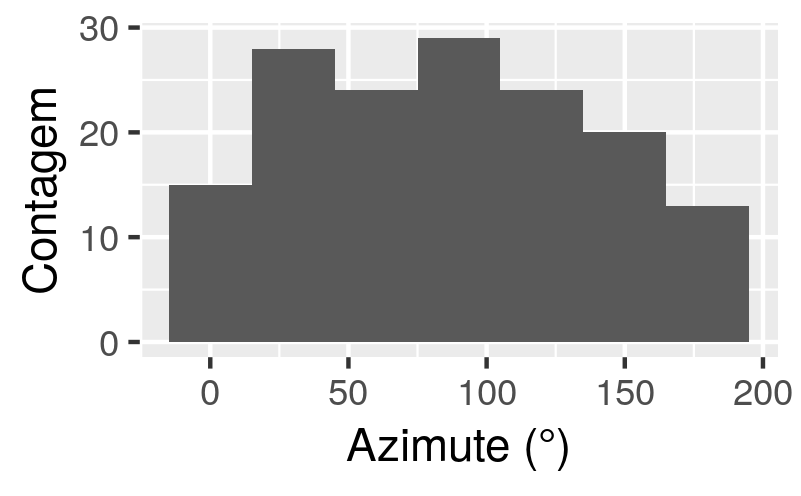
\includegraphics[width=\linewidth]{img/hist_azimute.png}
		\end{minipage}%
		\begin{minipage}{.5\textwidth}
			\centering
			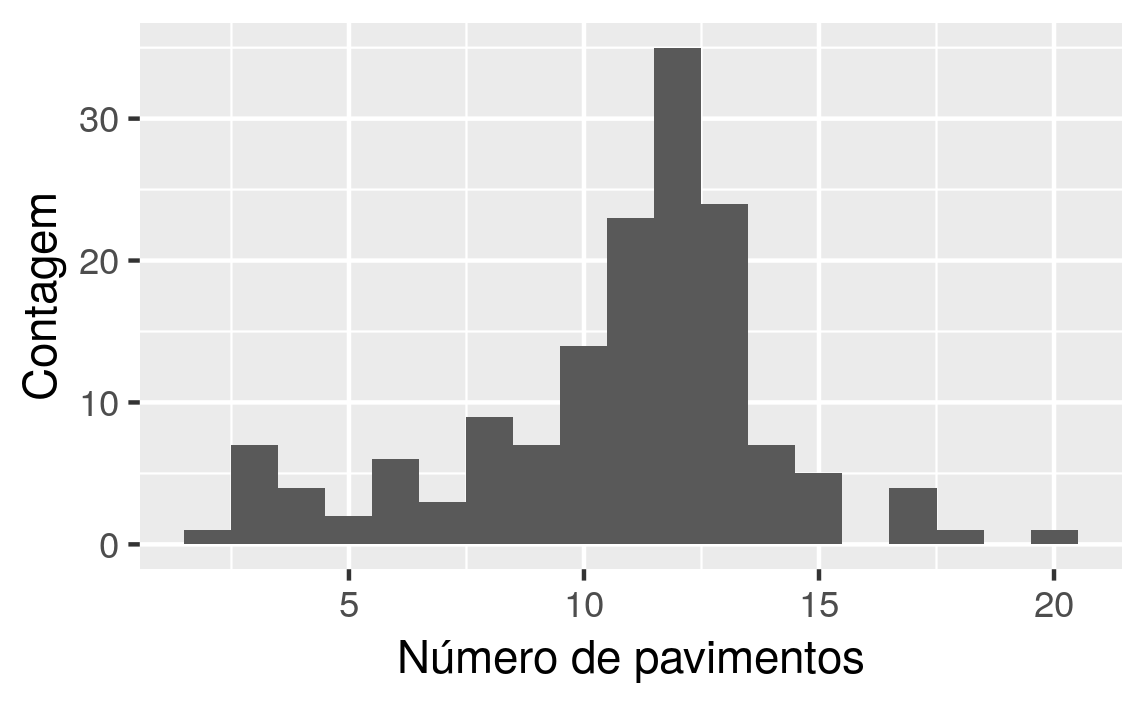
\includegraphics[width=\linewidth]{img/hist_numero_pavimentos.png}
		\end{minipage}
		\centering
		\begin{minipage}{.5\textwidth}
			\centering
			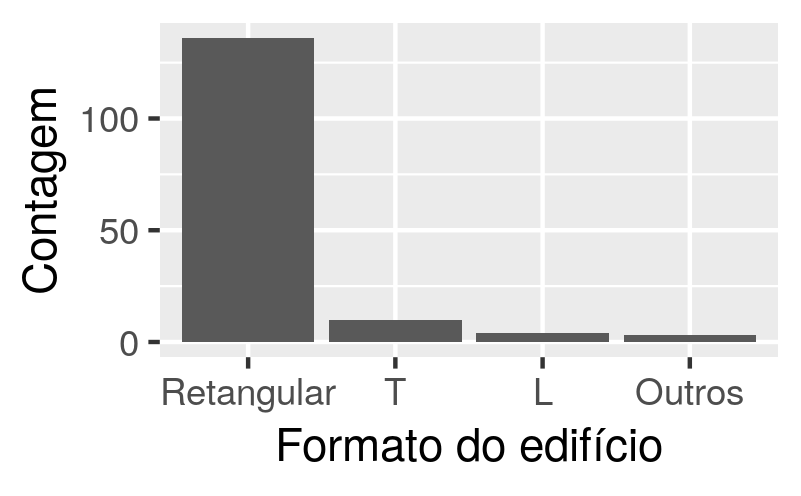
\includegraphics[width=\linewidth]{img/hist_formato.png}
		\end{minipage}%
		\begin{minipage}{.5\textwidth}
			\centering
			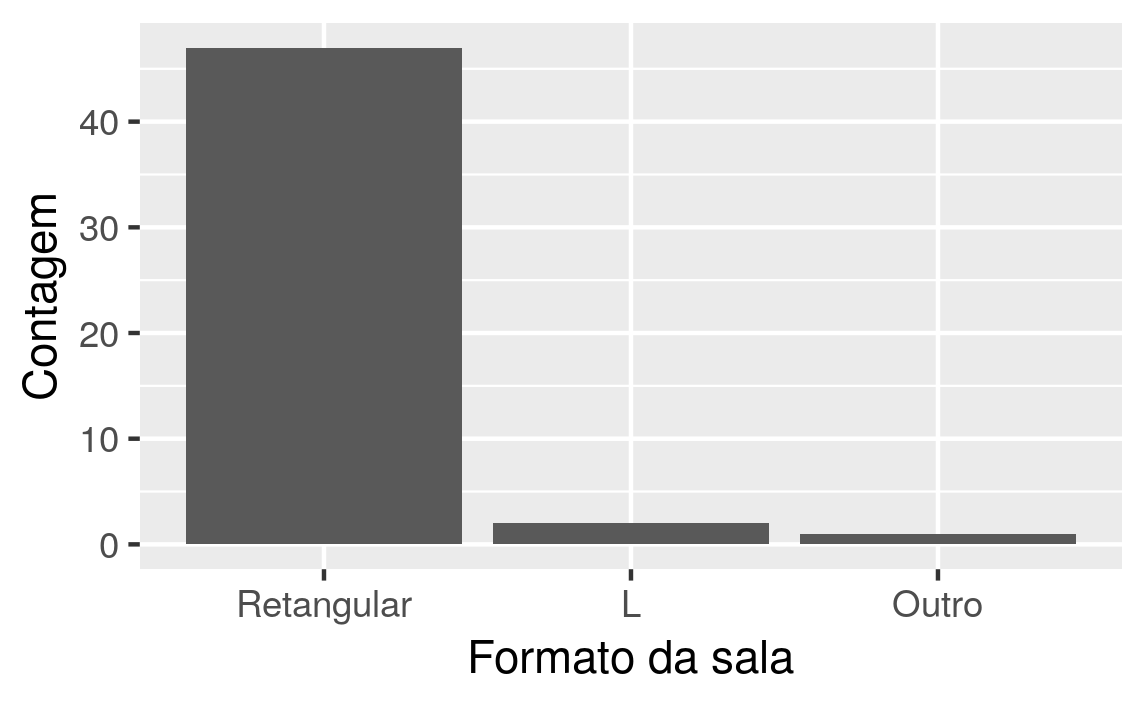
\includegraphics[width=\linewidth]{img/hist_formato_sala.png}
		\end{minipage}
		\centering
		\begin{minipage}{.5\textwidth}
			\centering
			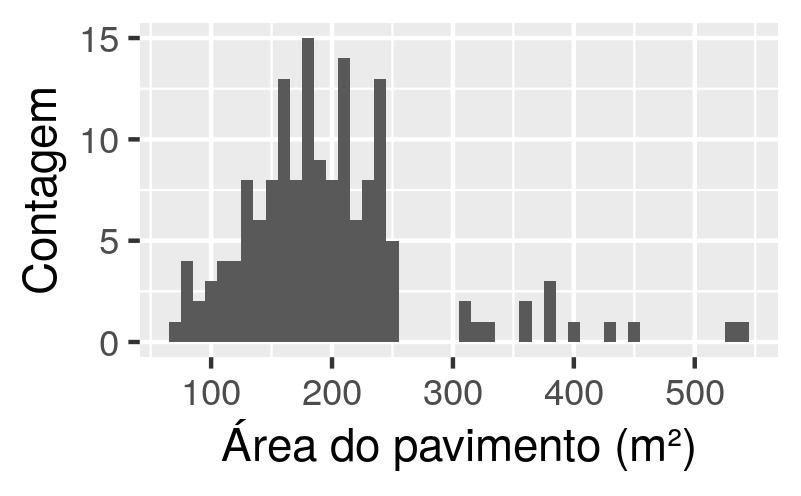
\includegraphics[width=\linewidth]{img/hist_area_edificio.png}
		\end{minipage}%
		\begin{minipage}{.5\textwidth}
			\centering
			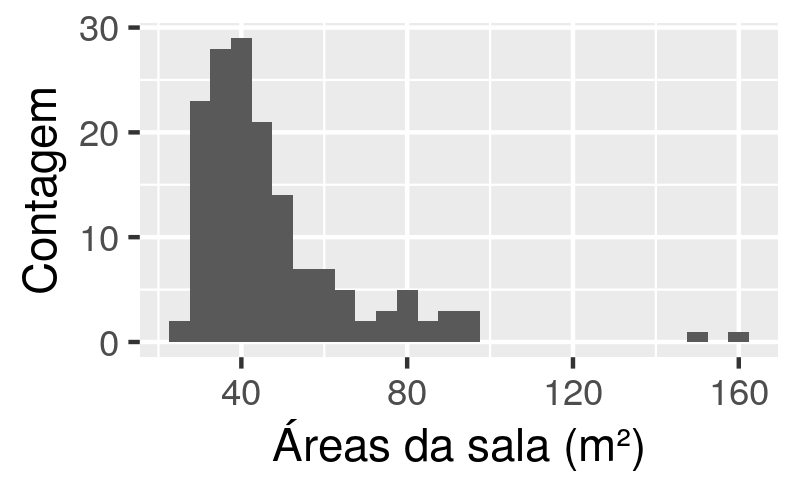
\includegraphics[width=\linewidth]{img/hist_area_zonas.png}
		\end{minipage}
		\centering
		\begin{minipage}{.5\textwidth}
			\centering
			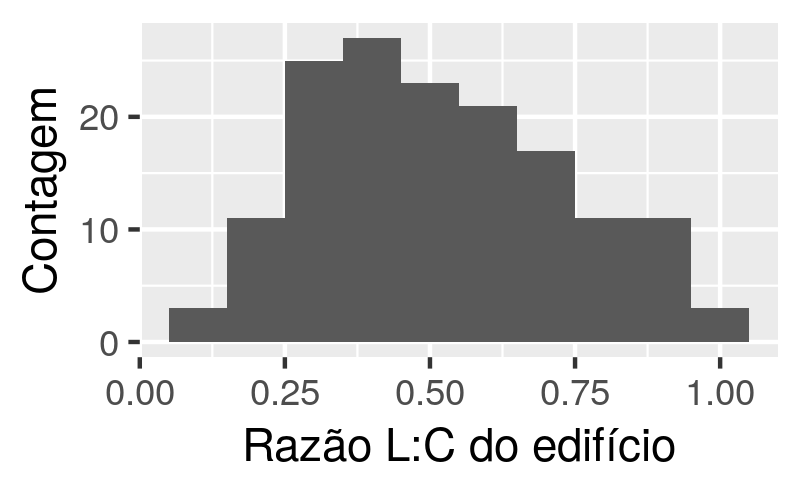
\includegraphics[width=\linewidth]{img/hist_ratio_edificio.png}
		\end{minipage}%
		\begin{minipage}{.5\textwidth}
			\centering
			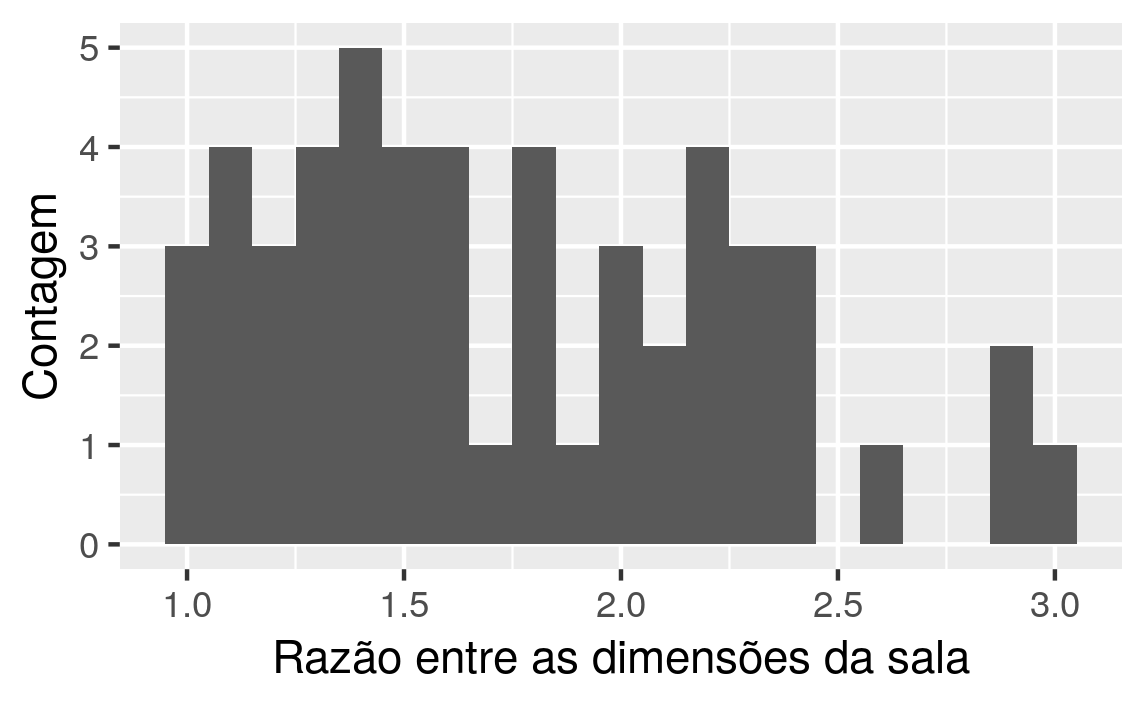
\includegraphics[width=\linewidth]{img/hist_ratio_sala.png}
		\end{minipage}
	\end{figure}
	\begin{figure}
		\captionof{figure}{Continuação}
		\label{fig:db_hist}
		\centering	
		\begin{minipage}{.5\textwidth}
			\centering
			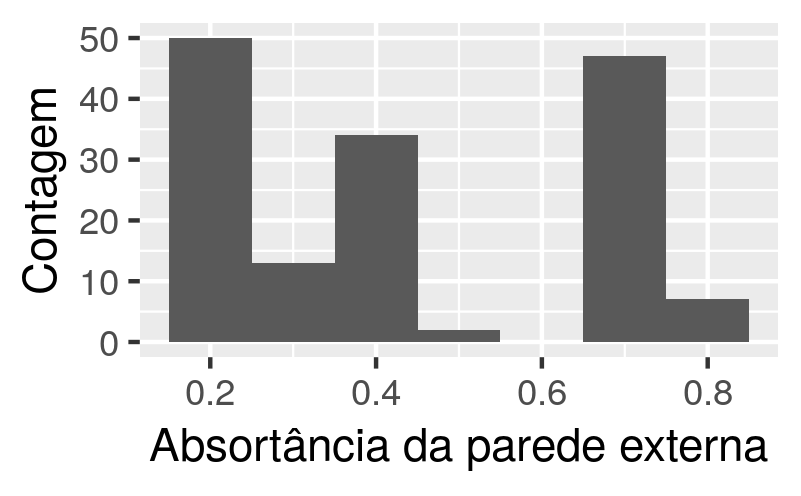
\includegraphics[width=\linewidth]{img/hist_absortancia.png}
		\end{minipage}%
		\begin{minipage}{.5\textwidth}
			\centering
			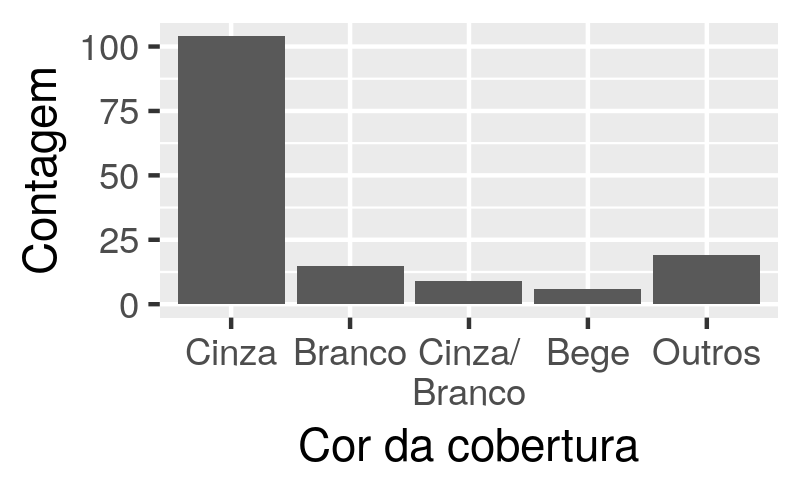
\includegraphics[width=\linewidth]{img/hist_cor_cobertura.png}
		\end{minipage}
		\centering	
		\begin{minipage}{.5\textwidth}
			\centering
			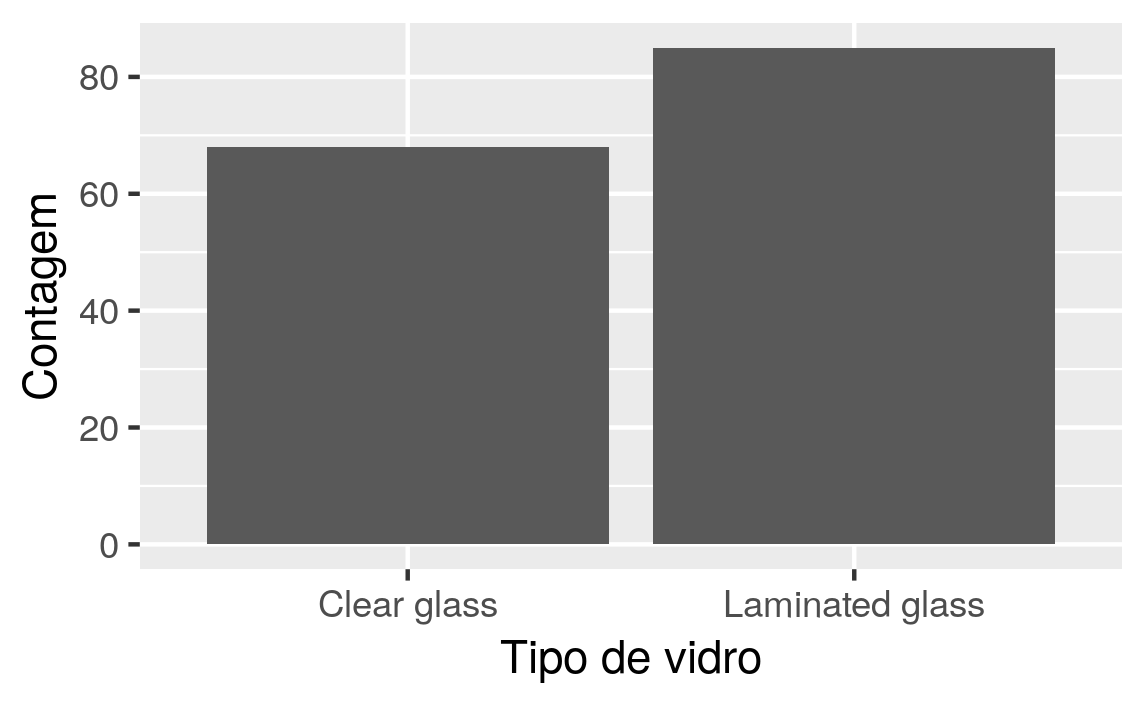
\includegraphics[width=\linewidth]{img/hist_tipo_vidro.png}
		\end{minipage}%
		\begin{minipage}{.5\textwidth}
			\centering
			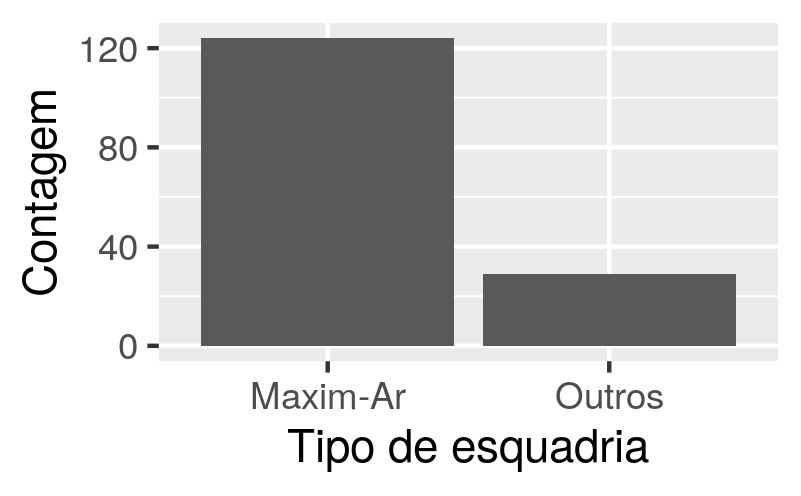
\includegraphics[width=\linewidth]{img/hist_esquadria.png}
		\end{minipage}
		\centering	
		\begin{minipage}{.5\textwidth}
			\centering
			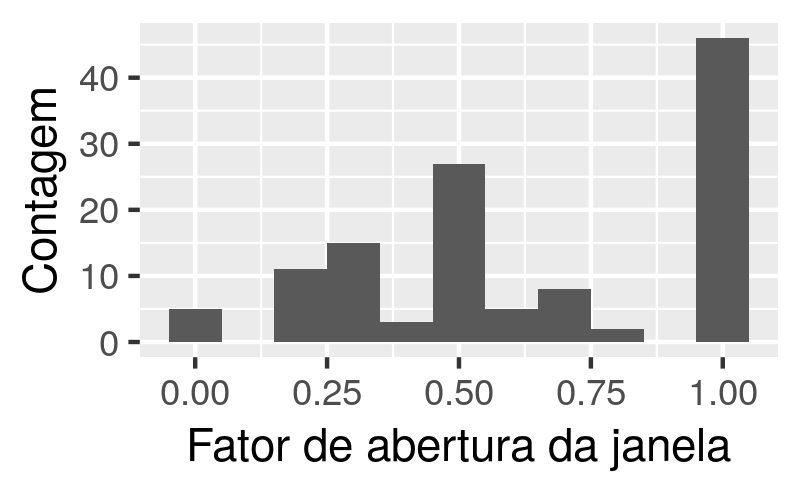
\includegraphics[width=\linewidth]{img/hist_openfac.png}
		\end{minipage}%
		\begin{minipage}{.5\textwidth}
			\centering
			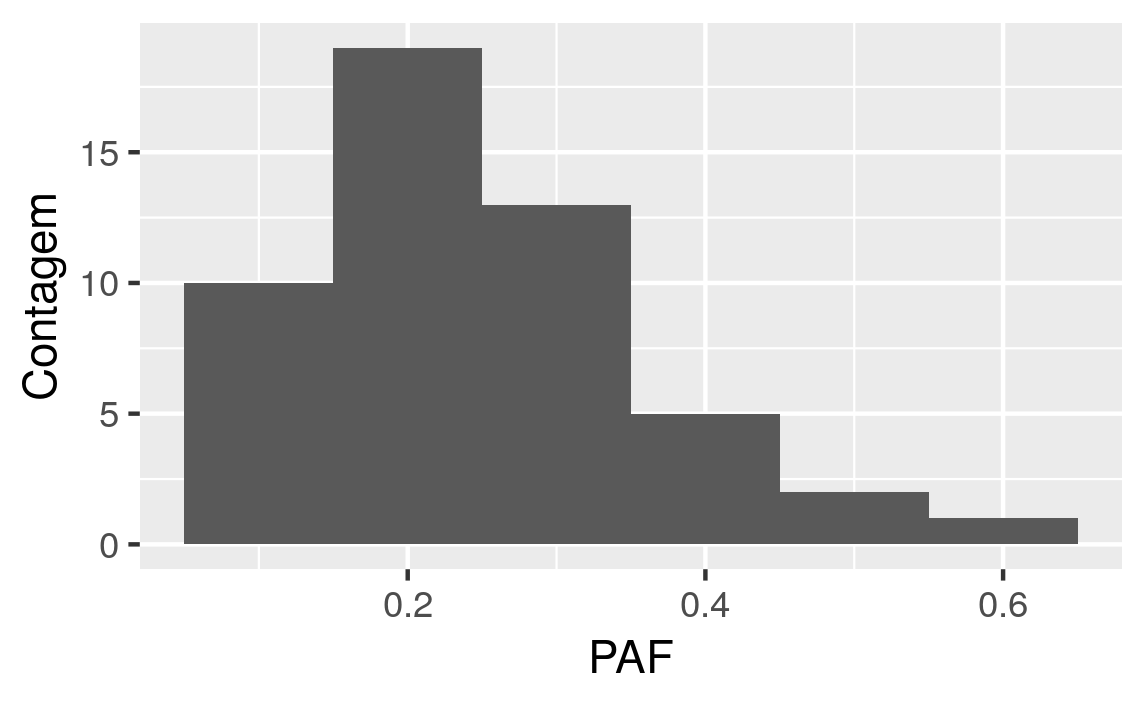
\includegraphics[width=\linewidth]{img/hist_PAF.png}
		\end{minipage}
		\centering	
		\begin{minipage}{.5\textwidth}
			\centering
			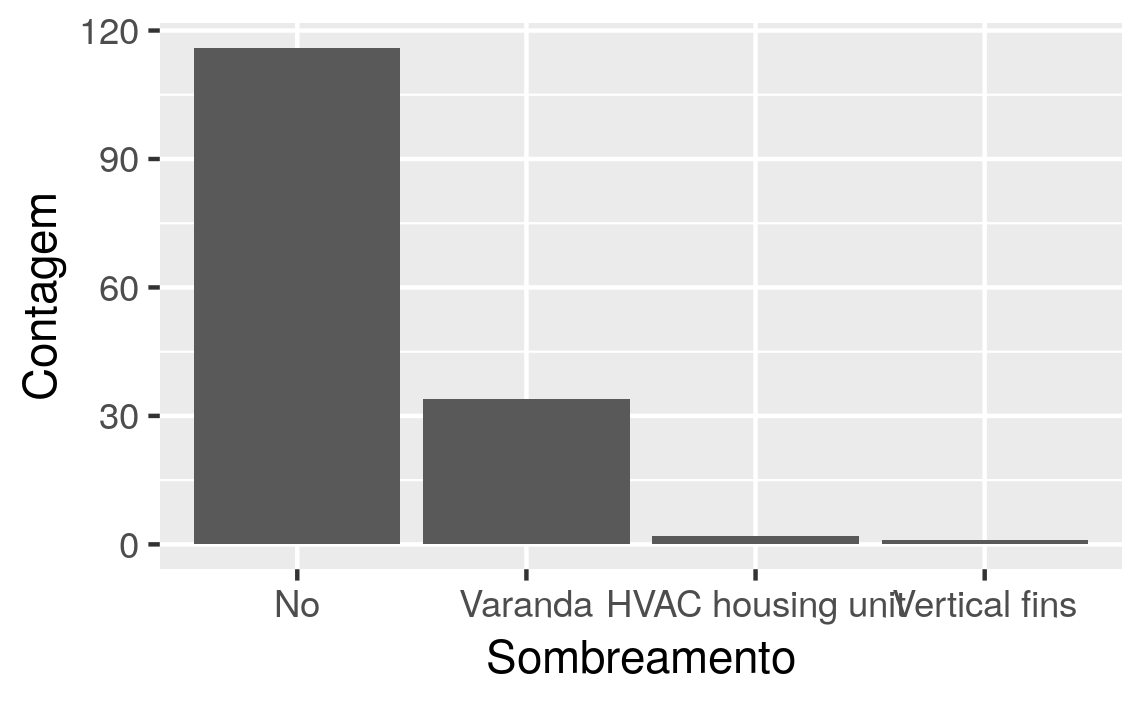
\includegraphics[width=\linewidth]{img/hist_sombreamento.png}
		\end{minipage}%
		\begin{minipage}{.5\textwidth}
			\centering
			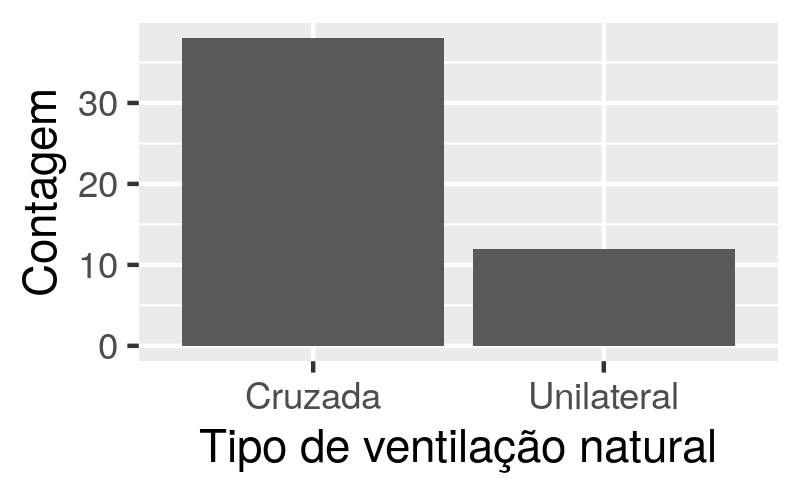
\includegraphics[width=\linewidth]{img/hist_tipo_vn.png}
		\end{minipage}
	\end{figure}
	
	Tanto os edifícios, quanto as salas existentes no banco de dados apresentam predominantemente formato retangular, a partir do qual considera-se que definir as simulações baseadas em modelos de edificações retangulares, como salas retangulares, representa adequadamente as tipologias de edifícios encontradas na cidade de São Paulo.
	
	A absortância da cobertura foi definida com o valor fixo de 0,7, valor aproximado para uma cobertura de cor cinza.
	
	Observou-se que esquadrias do tipo maxim-ar são predominante. Os objetos do \textit{Airflow Network} não modelam especificamente este tipo de esquadria. Porém, optou-se por considerar as janelas como não pivotantes. Considerar uma janela como horizontalmente pivotante implicaria na consideração de que a abertura acontece simultaneamente em cima e embaixo da janela. No caso da janela maxim-ar, por mais que a abertura aconteça em um eixo horizontal, ela abre apenas por baixo.
	
	O uso de elementos de sombreamento é pouco explorado nas edificações existentes. De qualquer maneira, considerou-se a modelagem de sombreamento horizontal sobre as aberturas da edificação, por considerar o potencial do sombreamento para bloquear a entrada de radiação nas zonas térmicas simuladas. Esse parâmetro foi variado a partir do ângulo de sombreamento formado entre a base da abertura e a proteção solar, localizada no topo da abertura.
	
	As informações relacionadas ao tipo de vidro não permitem definir valores relacionados ao fator solar. Observa-se apenas a ocorrência de vidros laminados e vidro comum incolor. Optou-se por variar o fator solar dos vidros nas simulações para avaliar o impacto deste parâmetro nos resultados de conforto térmico.
	
	A maioria das salas observadas possuem ventilação cruzada, mas a ventilação unilateral é uma estratégia com ocorrência considerável.
	
	Os demais parâmetros observados variaram continuamente de acordo com as distribuições obtidas. Como modelou-se apenas um pavimento nas simulações de referência, o parâmetro relacionado ao número de pavimento das edificações foi transformado no parâmetro "altura do pavimento".
	
	A Tabela \ref{table:param_def} apresenta os limites mínimos e máximos atribuídos aos diferentes parâmetros contínuos variados nas simulações, assim como os parâmetros variados pela lógica "sim/não". A velocidade do ar foi variada com valores discretos, de acordo com a Tabela \ref{table:var} do Capítulo \ref{chapter:metodologia}.
	
		\begin{table}[H]
			\centering
			\caption{Limites mínimos e máximos dos parâmetros}
			\label{table:param_def}
			\begin{tabular}{|l |r |}
				\hline
				\textbf{Parâmetro} & \textbf{Valores} \\
				\hline
				Área da sala (m$^2$) & 20 - 100 \\
				\hline
				Razão L:C da sala (-) & 0,4 - 2,5 \\
				\hline
				Pé-direito (m) & 2,3 - 3,2 \\
				\hline
				Azimute ($^{\circ}$) & 0 - 360 \\
				\hline
				Altura do pavimento (m) & 0 - 50 \\
				\hline 
				Absortância da parede (-) & 0,2 - 0,8 \\
				\hline 
				Transmitância da parede (W/m$^2$K) & 0,5 - 4,4 \\
				\hline 
				Capacidade térmica da parede (kJ/m$^2$K) & 0,22 - 450,00 \\
				\hline 
				PAF (-) & 0,1 - 0,6 \\
				\hline 
				Fator solar do vidro (-) & 0,20 - 0,87 \\
				\hline 
				Sombreamento ($^{\circ}$) & 0 - 80 \\
				\hline 
				Densidade de ocupação (pessoa/m$^2$) & 0,05 - 0,20 \\
				\hline 
				Fator de abertura da janela (-) & 0,2 - 1,0 \\
				\hline 
				Razão L:C do edifício (-) & 0,2 - 1,0 \\
				\hline 
				Cobertura exposta & Sim / Não\\
				\hline 
				Piso exposto & Sim / Não\\
				\hline 
				Ventilação & Cruzada / Unilateral\\
				\hline 
				Velocidade do ar (m/s) & 0,0 - 1,2 \\
				\hline 
			\end{tabular}
%			\begin{flushleft}
%				Fonte: \citeauthoronline{INIC} \cite{INIC}, adaptado pelo autor.
%			\end{flushleft}				
		\end{table}
		
		\section{Simulações simplificadas}
		
		\subsection{Cálculo do coeficiente de pressão pelo método analítico}
		
		Ao comparar os valores dos coeficientes de pressão (Cp’s) das medições em túnel de vento da Universidade Politécnica de Tóquio (TPU) e os valores dos Cp’s obtidos pelo método analítico (MA), obteve-se o gráficos de pontos. 
		A Figura \ref{fig:cp_diff_scatter_all} apresenta a comparação para as 25 geometrias diferentes, para cada fachada, e para cada ponto disponibilizado pela TPU.
		Como os valores calculados pelo MA são únicos para cada fachada, e a TPU oferece valores diferentes para diversos pontos ao longo das fachadas, os pontos no gráfico da Figura \ref{fig:cp_diff_scatter_all} distribuem-se horizontalmente. 
%		A Figura \ref{fig:cp_diff_scatter_facade} apresenta a comparação considerando-se os valores médios do Cp para cada fachada. 
		É possível observar que a faixa de valores dos Cp's disponibilizados pela TPU é maior do que  faixa de valores calculados pelo MA. Enquanto o menor valor de Cp disponibilizado pela TPU é -1,40, e o maior valor é 1,08, pelo MA o valor mínimo é igual a -0,96 e o máximo é igual a 0,60.
		
		\begin{figure}[H]
			\centering
			\caption{Comparação entre os valores de Cp das 25 geometrias}
			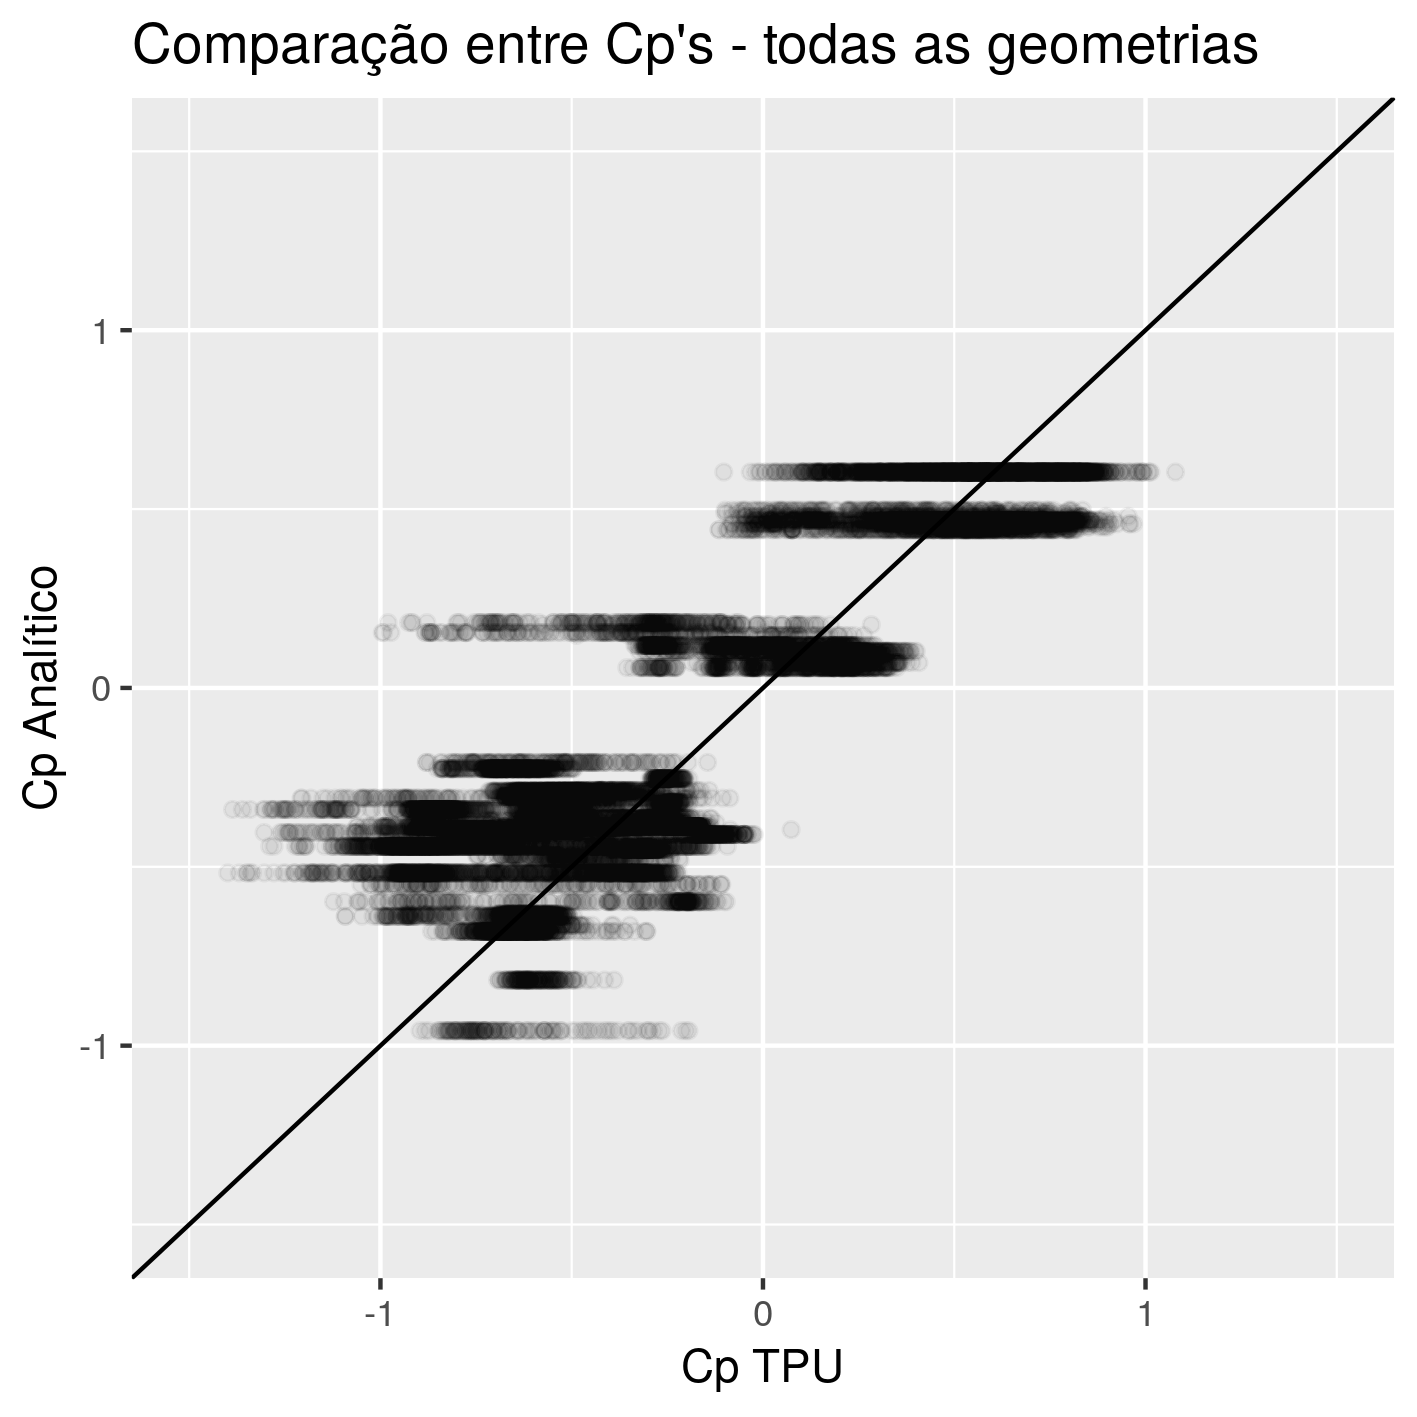
\includegraphics[width=1\linewidth]{img/cp_diff_scatter_all.png}
			\label{fig:cp_diff_scatter_all}
			%			\begin{flushleft}
			%				Fonte: o autor.
			%			\end{flushleft}
		\end{figure}
		
		Dentre as geometrias analisadas, a proporção com a maior diferença absoluta média entre os valores dos	Cp’s obtidos pela base da TPU e obtidos pelo MA foi igual a 0,344, para a geometria da edificação \textit{highrise} com proporções de largura, profundidade e altura igual a 2:1:2 (Figura \ref{fig:cp_diff_scatter}).
	
		\begin{figure}[H]
			\centering
			\caption{Comparação entre os valores de Cp da geometria de proporções 2:1:2}
			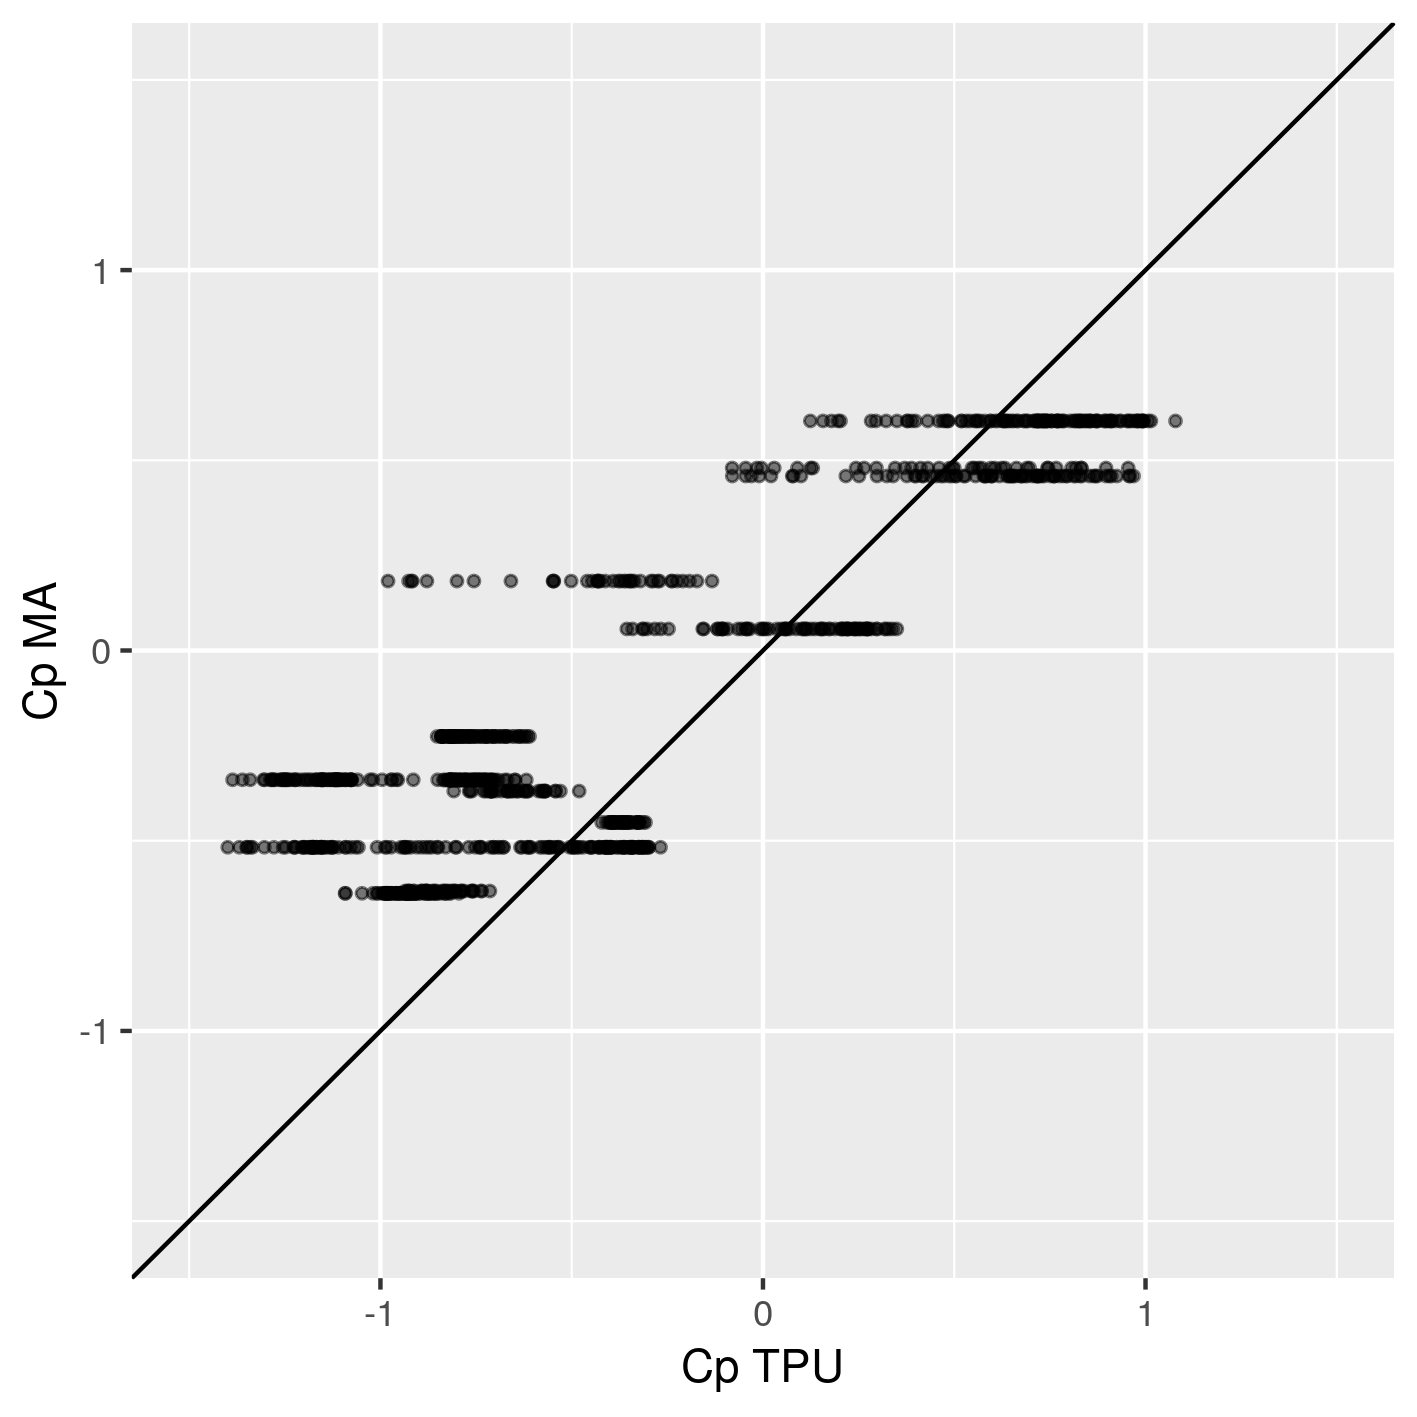
\includegraphics[width=1\linewidth]{img/cp_diff_scatter.png}
			\label{fig:cp_diff_scatter}
			%			\begin{flushleft}
			%				Fonte: o autor.
			%			\end{flushleft}
		\end{figure}
	
		A partir da comparação conduzida, decidiu-se comparar as diferenças nos resultados de simulações termoenergéticas utilizando como base uma tipologia com proporções de largura, profundidade e altura igual a 2:1:2.
		
		Os resultados das 1000 simulações foram comparados por gráficos de pontos. A comparação entre as médias das trocas de ar, apresentada na Figura \ref{fig:cpaverage_ACH_scatter}, mostra que o MA faz com que as simulações subestimem as trocas de ar nas simulações, possivelmente devido aos menores valores dos Cp's obtidos pelo método.
		A diferença média das trocas de ar foi igual a -0,67 trocas de ar por hora (ACH), com o erro absoluto do 95º percentil (AE95) é igual a 5,23 ACH.
		
		\begin{figure}[H]
			\centering
			\caption{Comparação entre as médias das ACH}
			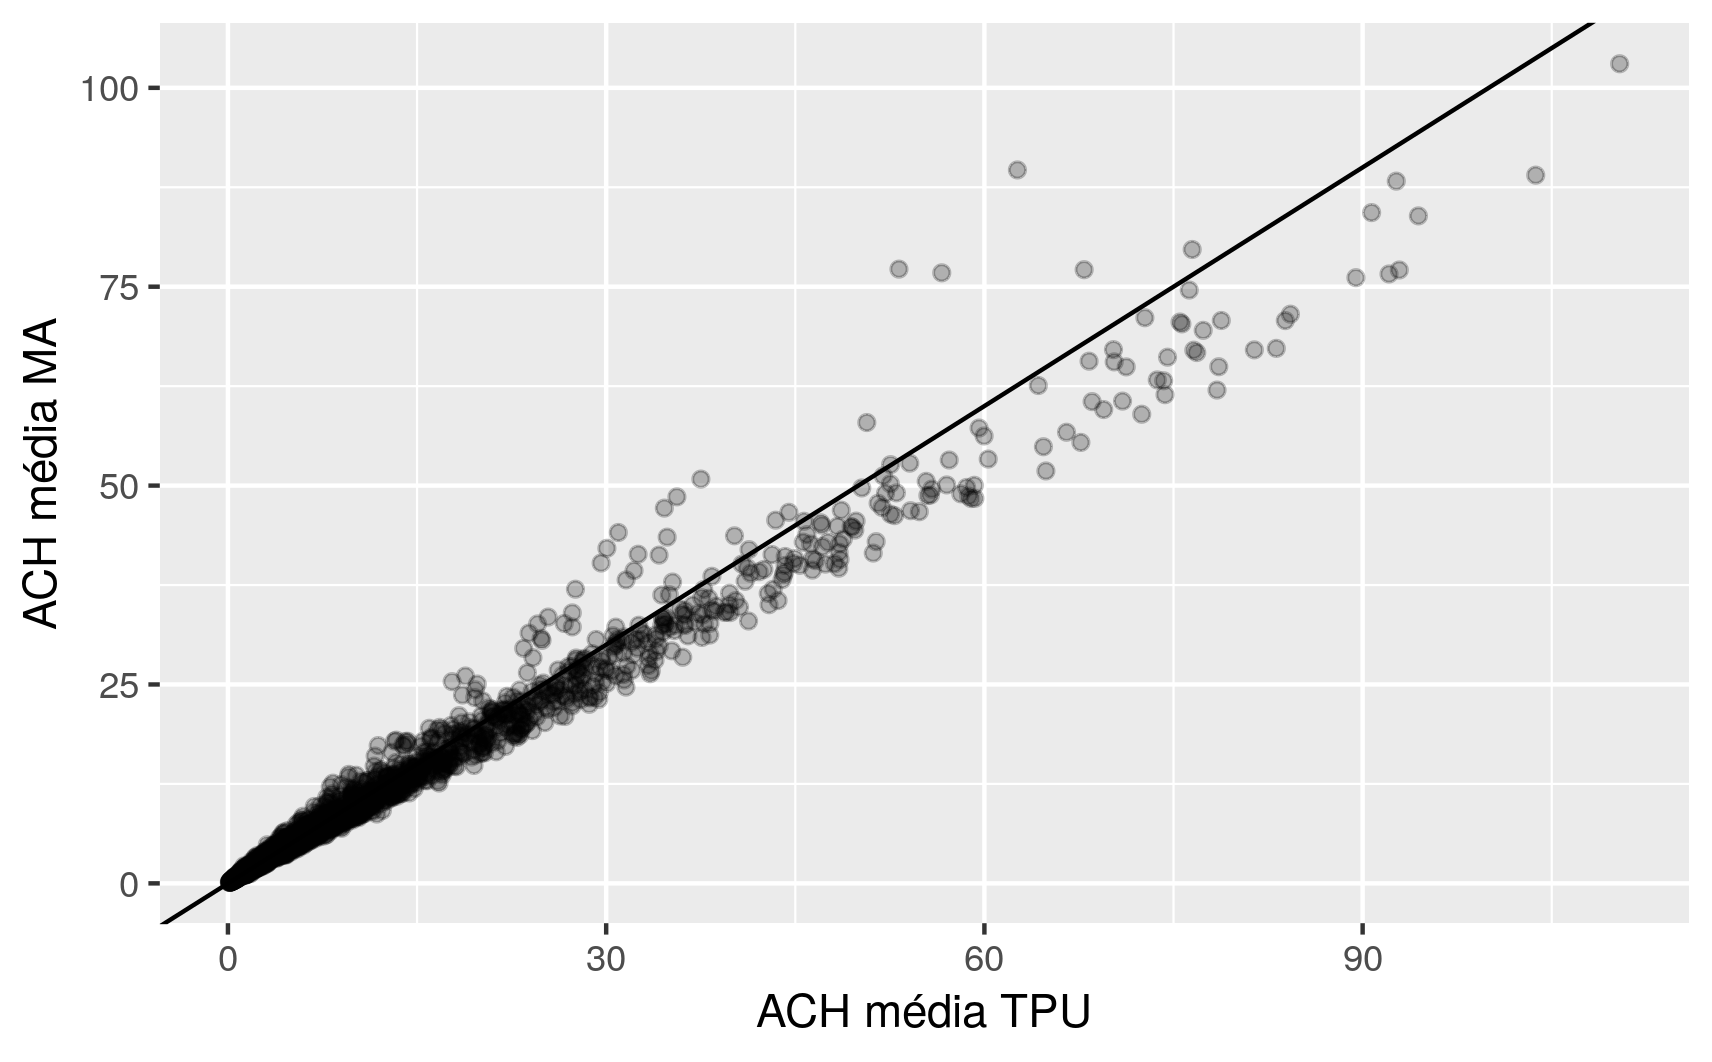
\includegraphics[width=1\linewidth]{img/cpaverage_ACH_scatter.png}
			\label{fig:cpaverage_ACH_scatter}
			%			\begin{flushleft}
			%				Fonte: o autor.
			%			\end{flushleft}
		\end{figure}
		
		Apesar dessas diferenças nas trocas de ar, a comparação entre as temperaturas operativas médias, apresentada na Figura \ref{fig:cpaverage_temp_scatter}, mostra que a diferença média da temperatura operativa é 0,04 $^{\circ}$C, sendo que o AE95 é igual a 0,31 $^{\circ}$C.
		Essas diferenças são confirmadas como pouco significativas ao se analisar o a Figura \ref{fig:cpaverage_EHF_scatter}, com a comparação da fração de horas em desconforto (EHF). A média de diferença do EHF nos casos analisados foi igual a 0,0037, com o AE95 igual a 0,0277.
		Por tanto, considerou-se que a utilização do MA para calcular os valores dos Cp's é uma alternativa adequada para a simplificação das simulações termoenergéticas.
		
		\begin{figure}[H]
			\centering
			\caption{Comparação entre as médias das temperaturas operativas}
			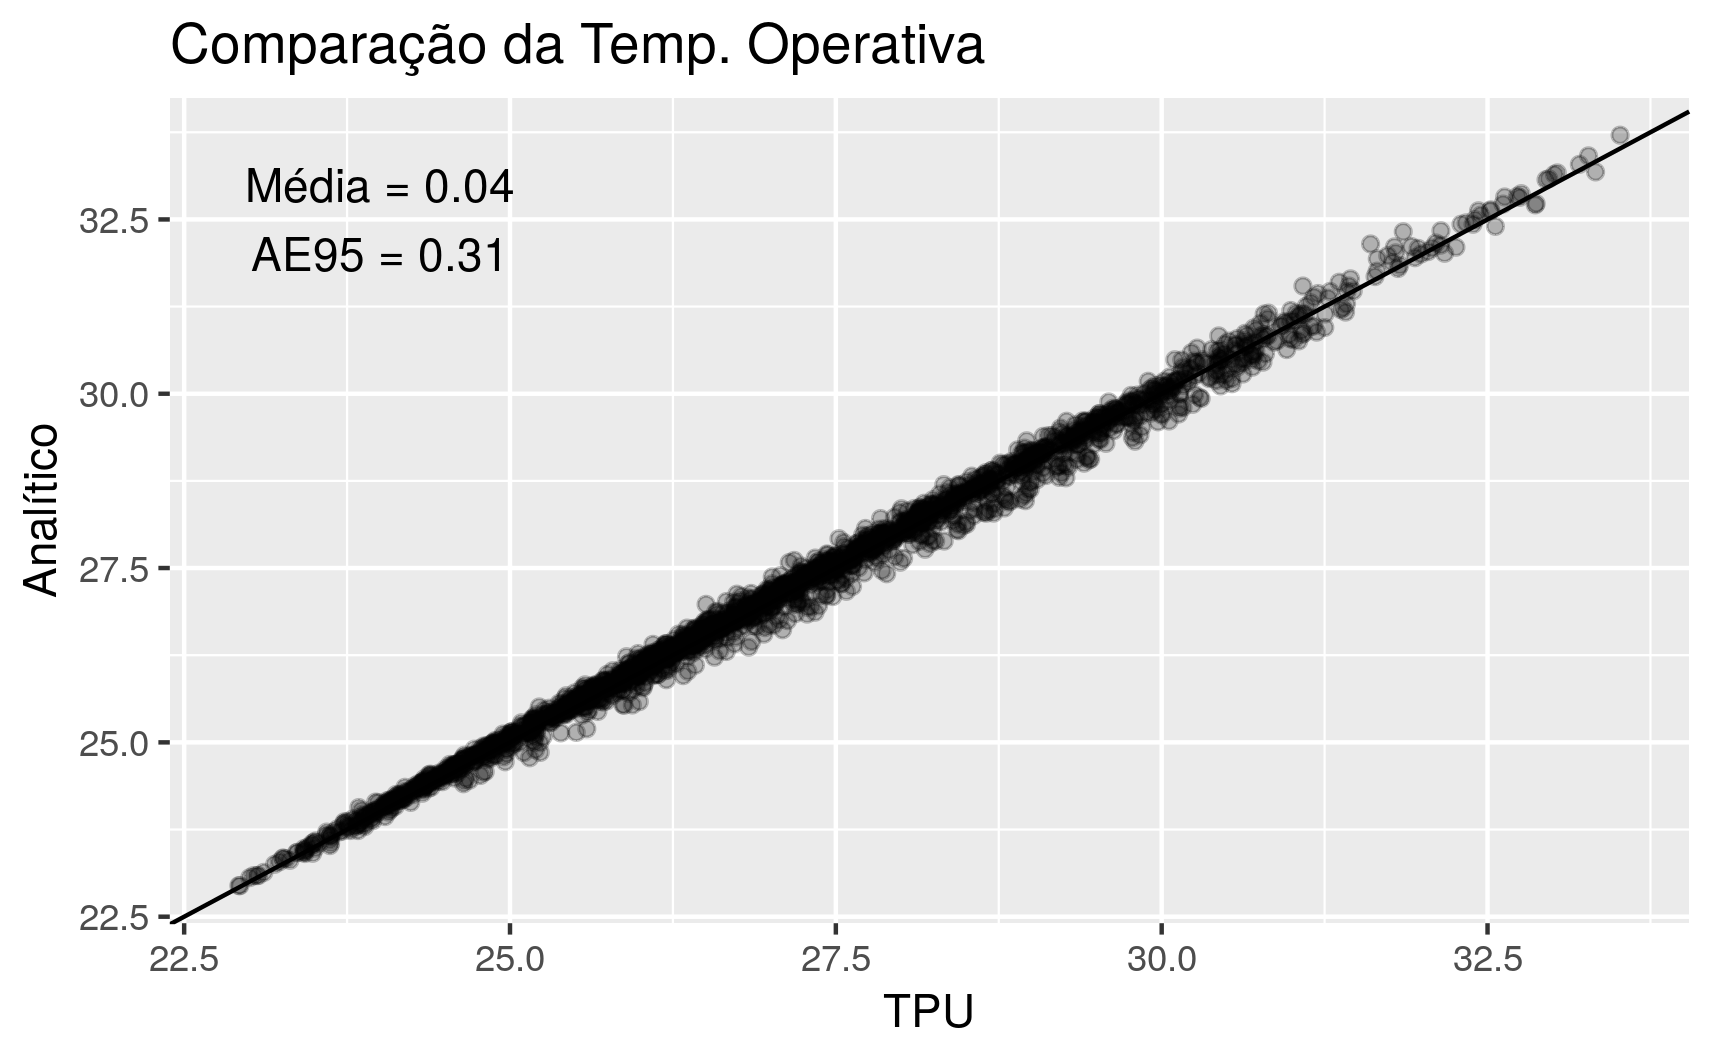
\includegraphics[width=1\linewidth]{img/cpaverage_temp_scatter.png}
			\label{fig:cpaverage_temp_scatter}
			%			\begin{flushleft}
			%				Fonte: o autor.
			%			\end{flushleft}
		\end{figure}
	
		\begin{figure}[H]
			\centering
			\caption{Comparação entre os resultados de EHF}
			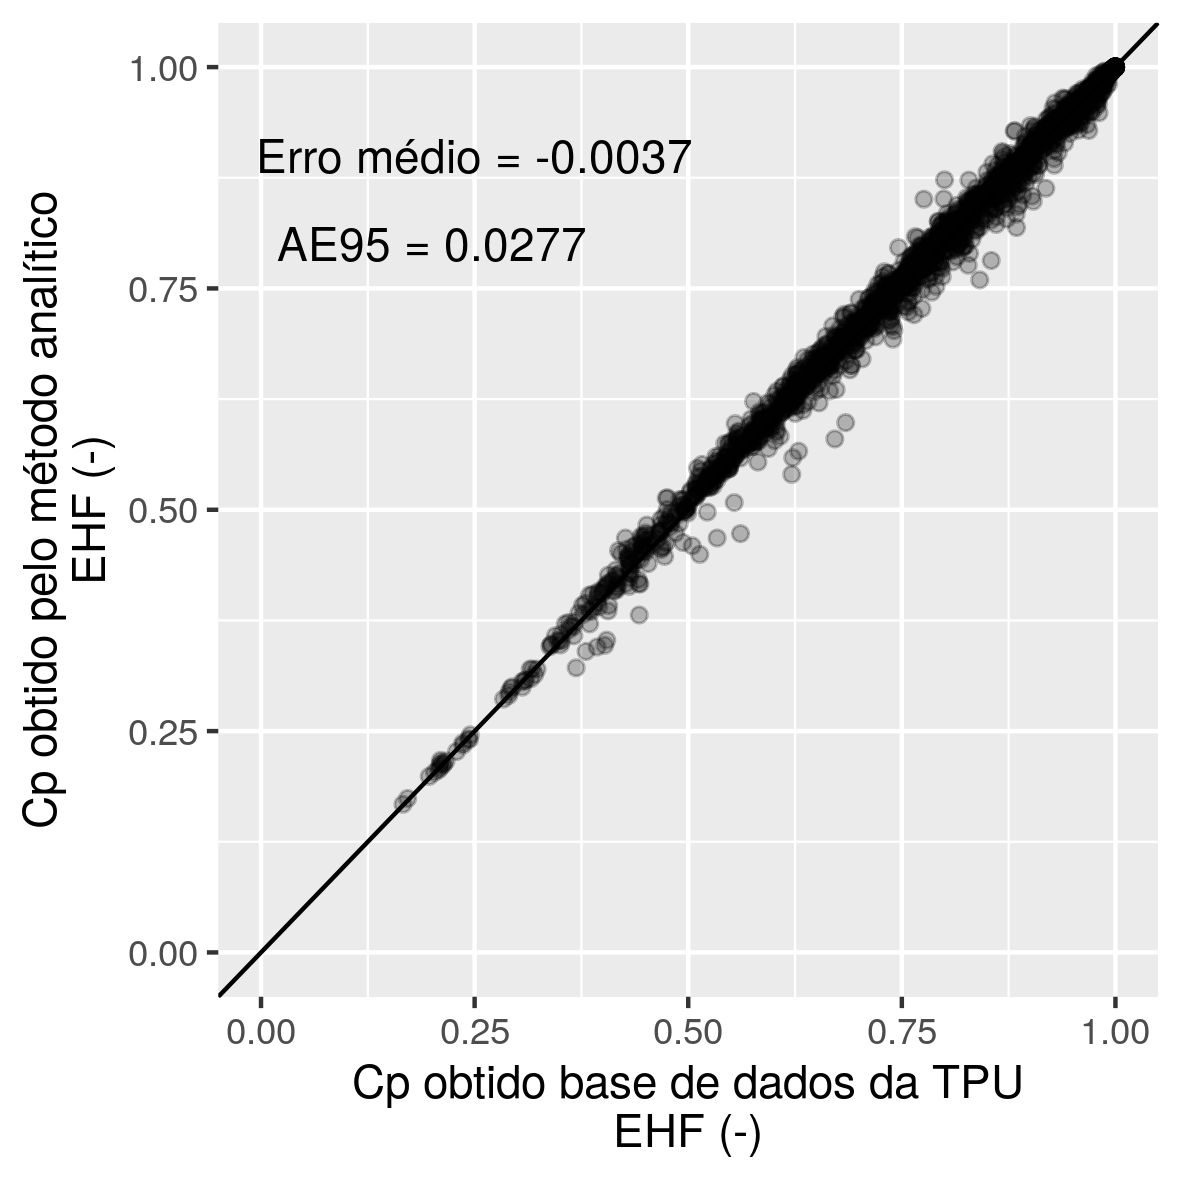
\includegraphics[width=1\linewidth]{img/cpaverage_EHF_scatter.png}
			\label{fig:cpaverage_EHF_scatter}
			%			\begin{flushleft}
			%				Fonte: o autor.
			%			\end{flushleft}
		\end{figure}
	
	\subsection{Representação da envoltória com duas camadas}
		
		Os resultados das simulações com as paredes equivalentes subestimaram o EHF em 0,0107 na média, quando comparados aos resultados das simulações com as paredes de referência. 
		Os resultados das simulações para a parede de gesso com isolamento mostram que o EHF é subestimado em um valor médio de 0,0099. Os resultados de EHF obtiveram um erro absolto médio igual a 0,0100, e um AE95 igual a 0,0604 (Figura \ref{fig:par3_scatter}).
		
		\begin{figure}[H]
			\centering
			\caption{Comparação entre os resultados de EHF para a parede de gesso com isolamento}
			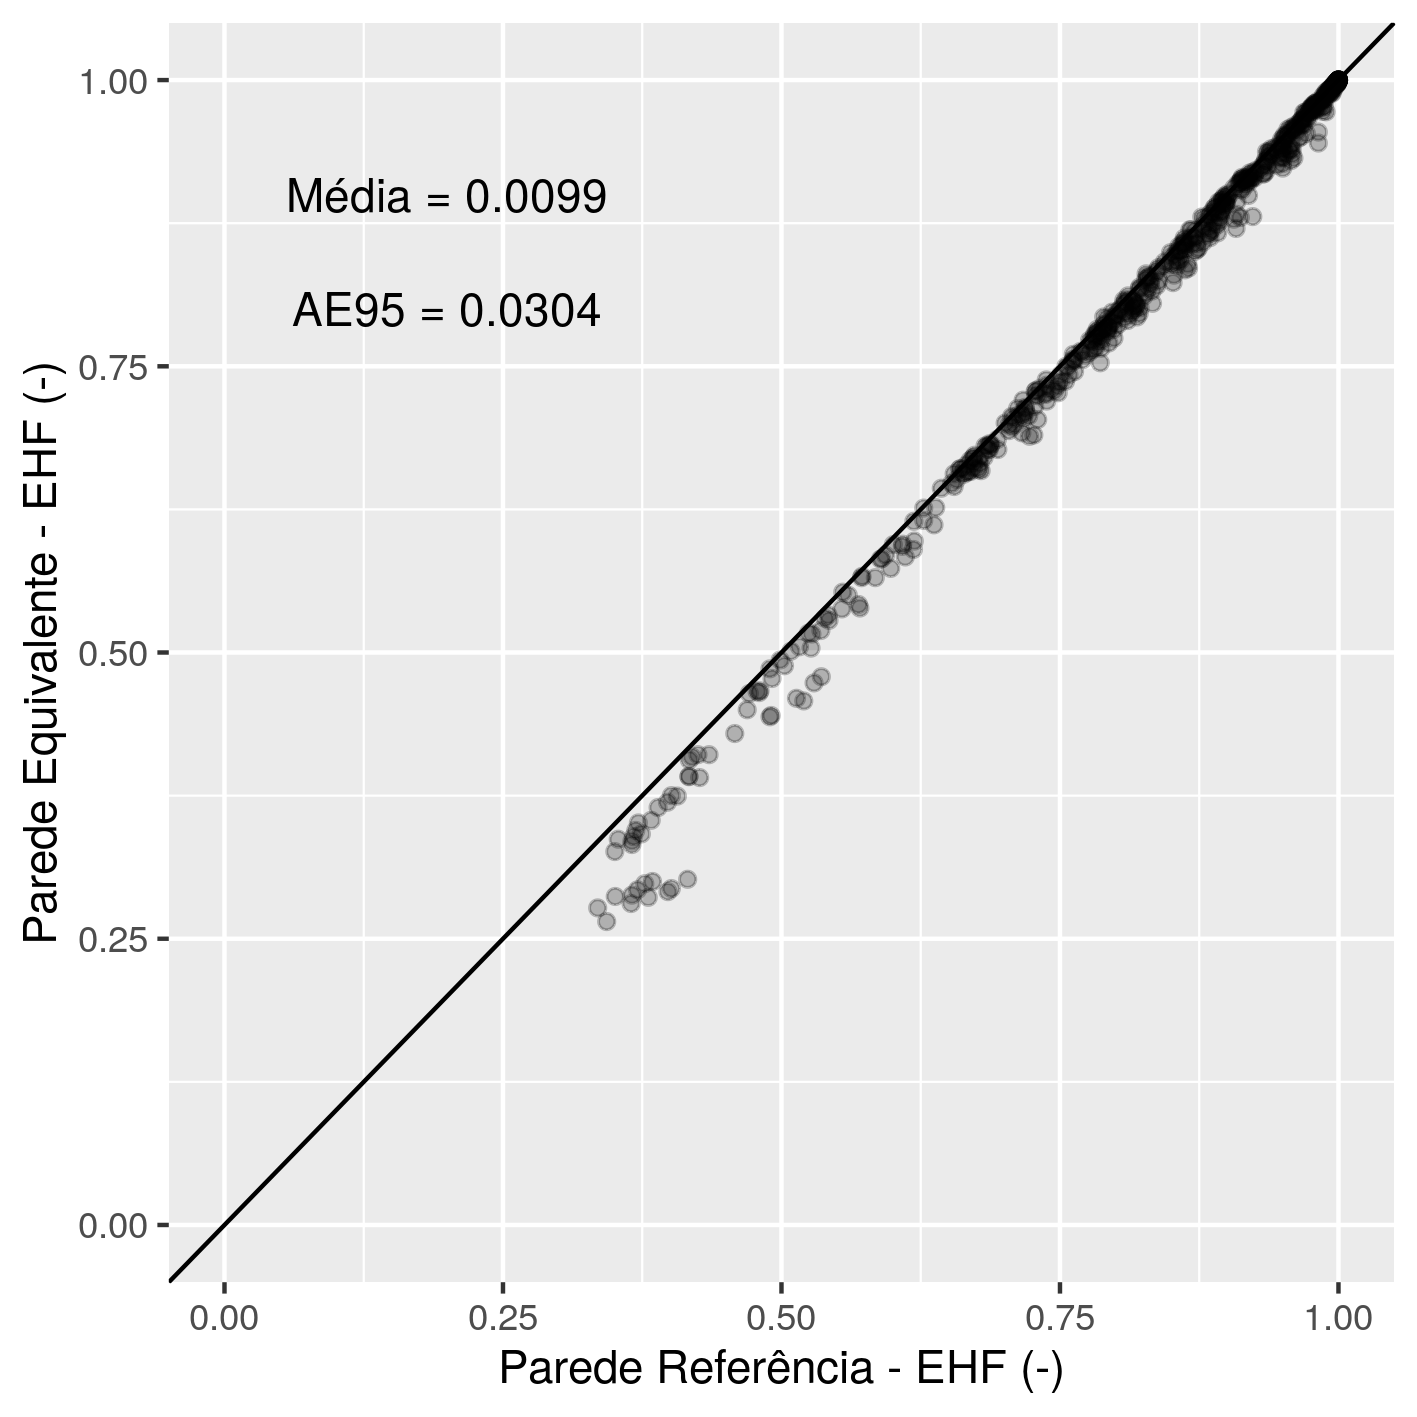
\includegraphics[width=1\linewidth]{img/paredeeq_EHF_par3_scatter.png}
			\label{fig:par3_scatter}
			%			\begin{flushleft}
			%				Fonte: o autor.
			%			\end{flushleft}
		\end{figure}
		
		A representação da parede de alvenaria apresenta-se mais adequada considerando-se apenas metade da parede para definir a capacidade térmica. Enquanto que, para a parede com a capacidade térmica total o erro absoluto médio foi igual a 0,0209, e o AE95 foi igual a 0,0650, para a parede de alvenaria com metade da capacidade térmica considerada, o erro médio absoluto foi igual a 0,0189, e o AE95 foi igual a 0,0604.
		
		\begin{figure}[H]
			\centering
			\caption{Comparação entre os resultados de EHF para a parede de alvenaria com capacidade térmica total}
			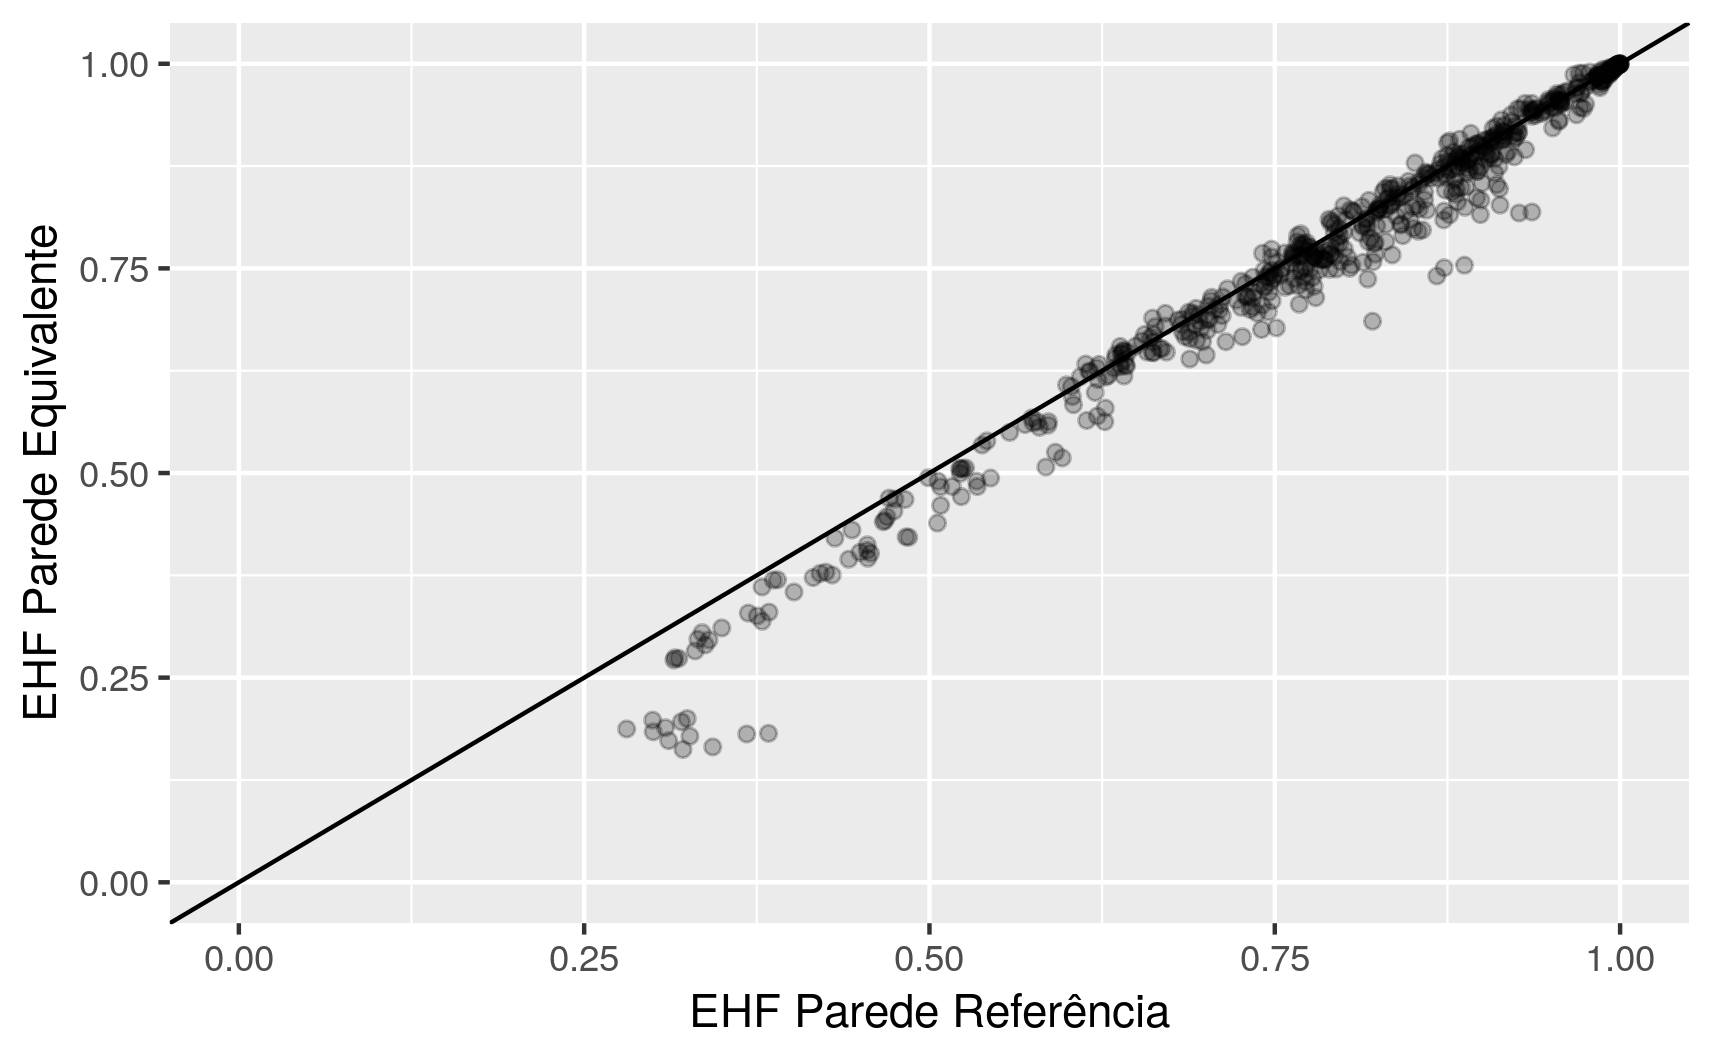
\includegraphics[width=1\linewidth]{img/paredeeq_EHF_par2a_scatter.png}
			\label{fig:par2a_scatter}
			%			\begin{flushleft}
			%				Fonte: o autor.
			%			\end{flushleft}
		\end{figure}
		\begin{figure}[H]
			\centering
			\caption{Comparação entre os resultados de EHF para a parede de alvenaria com metade da capacidade térmica}
			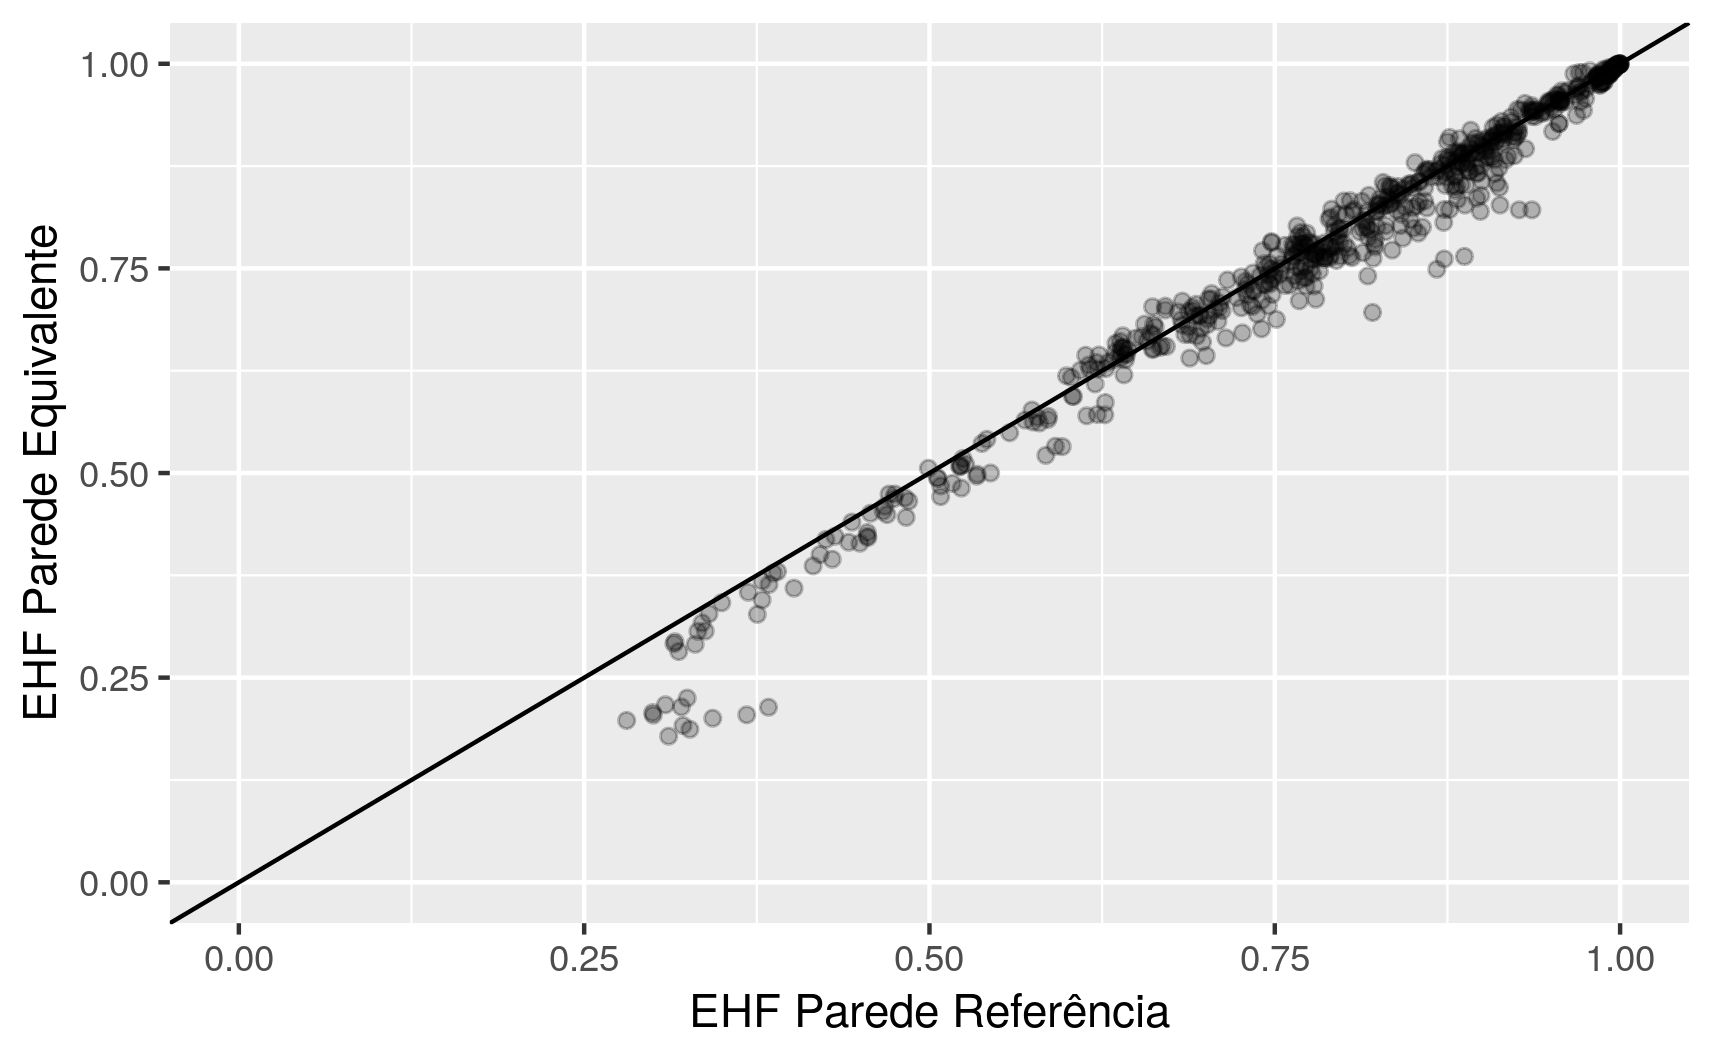
\includegraphics[width=1\linewidth]{img/paredeeq_EHF_par2b_scatter.png}
			\label{fig:par2b_scatter}
			%			\begin{flushleft}
			%				Fonte: o autor.
			%			\end{flushleft}
		\end{figure}
		
		O caso com as maiores diferenças no EHF foi para uma edificação em contato com o solo, com cobertura exposta, e um fator de abertura da janela igual a 0,23.
		Apesar das diferenças nos resultados, o uso da parede equivalente facilita a parametrização da transmitância térmica e da capacidade térmica. Por esse motivo, considerou-se as diferenças pouco significativas, e a parede equivalente foi adotada para simplificar as simulações.
		
		\subsection{Condição de contorno das paredes adjacentes à edificação}
		
		A simplificação das simulações adotando-se uma zona térmica foi avaliada para duas condições de contorno. Os resultados mostram que a maneira mais adequada de representar as paredes adjacentes à circulação da edificação é considerando-as como adiabáticas. Considerar as paredes adjacentes à circulação como \textit{Outdoors}, faz com que os resultados do EHF seja subestimados em 0,0868 em média, como AE95 igual a 0,1865 (Figura \ref{fig:szout_EHF}).
		
		\begin{figure}[H]
			\centering
			\caption{Comparação entre os resultados de EHF para parede \textit{Outdoors}}
			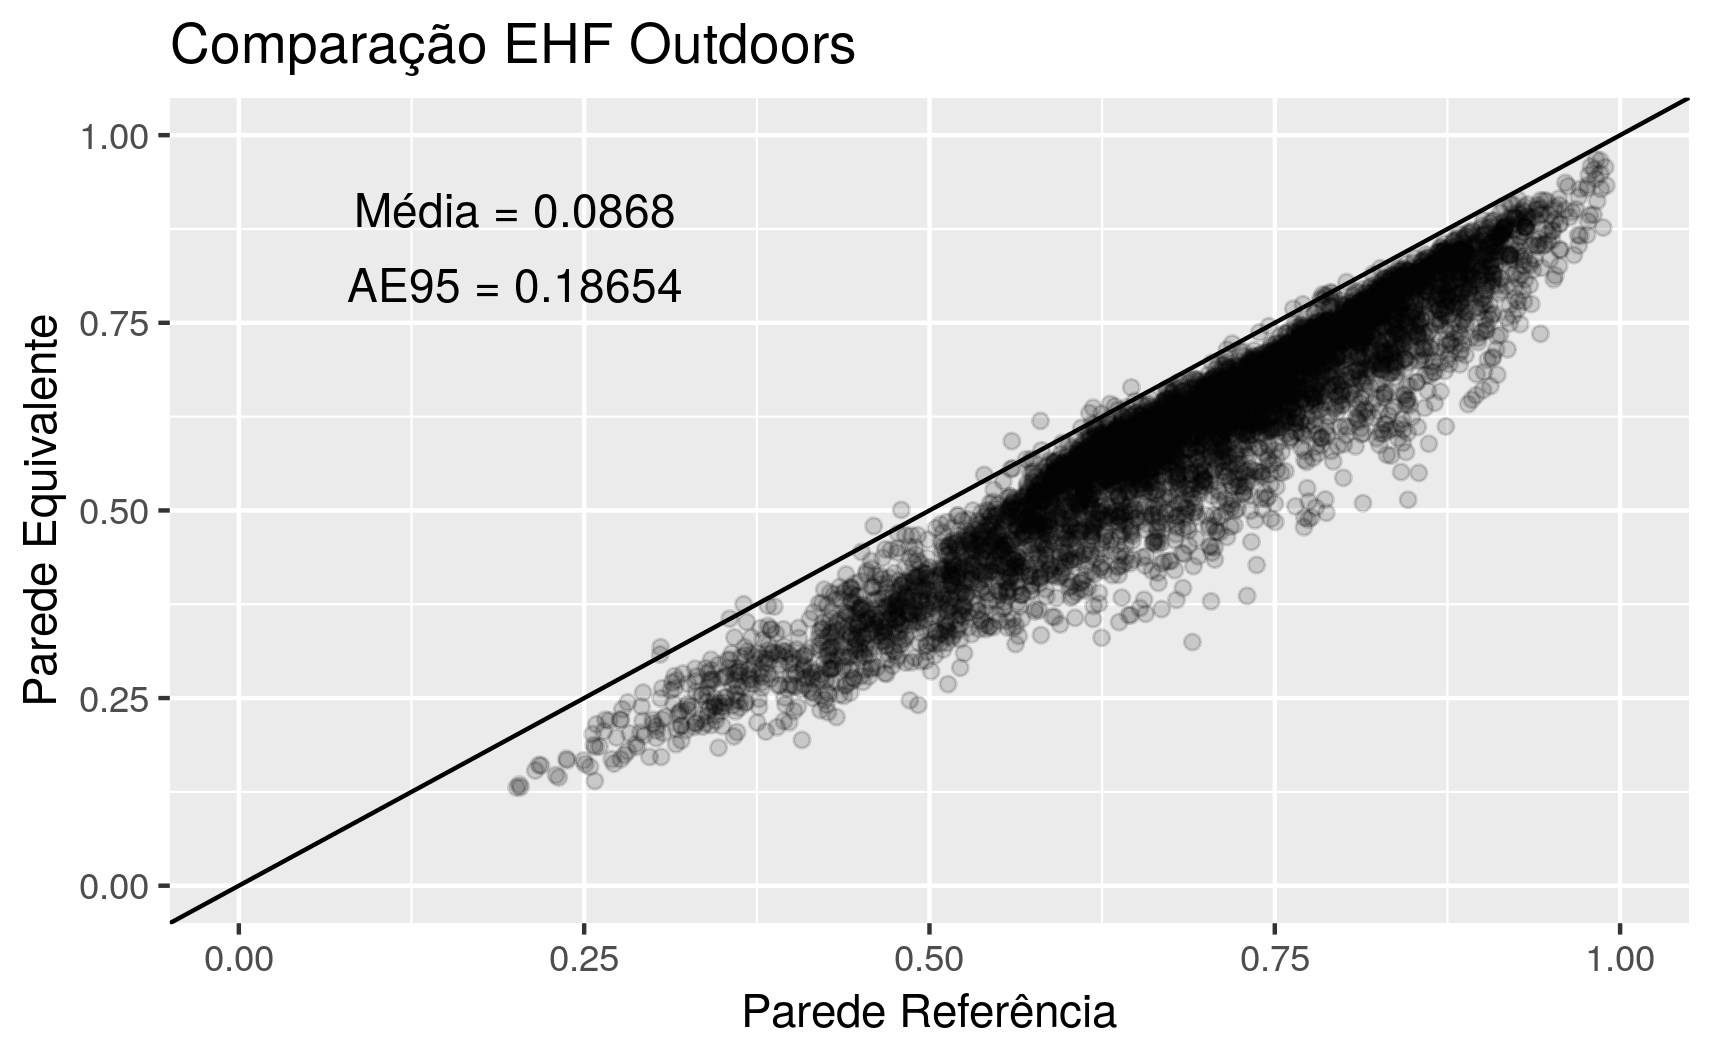
\includegraphics[width=1\linewidth]{img/szout_EHF_scatter.png}
			\label{fig:szout_EHF}
			%			\begin{flushleft}
			%				Fonte: o autor.
			%			\end{flushleft}
		\end{figure}
		
		Os resultados das simulações considerando-se as paredes voltadas para o corredor como adiabáticas subestimaram o EHF em 0,0051 na média, como AE95 igual a 0,0804 (Figura \ref{fig:szadi_EHF}).
		
		\begin{figure}[H]
			\centering
			\caption{Comparação entre os resultados de EHF para parede adiabática}
			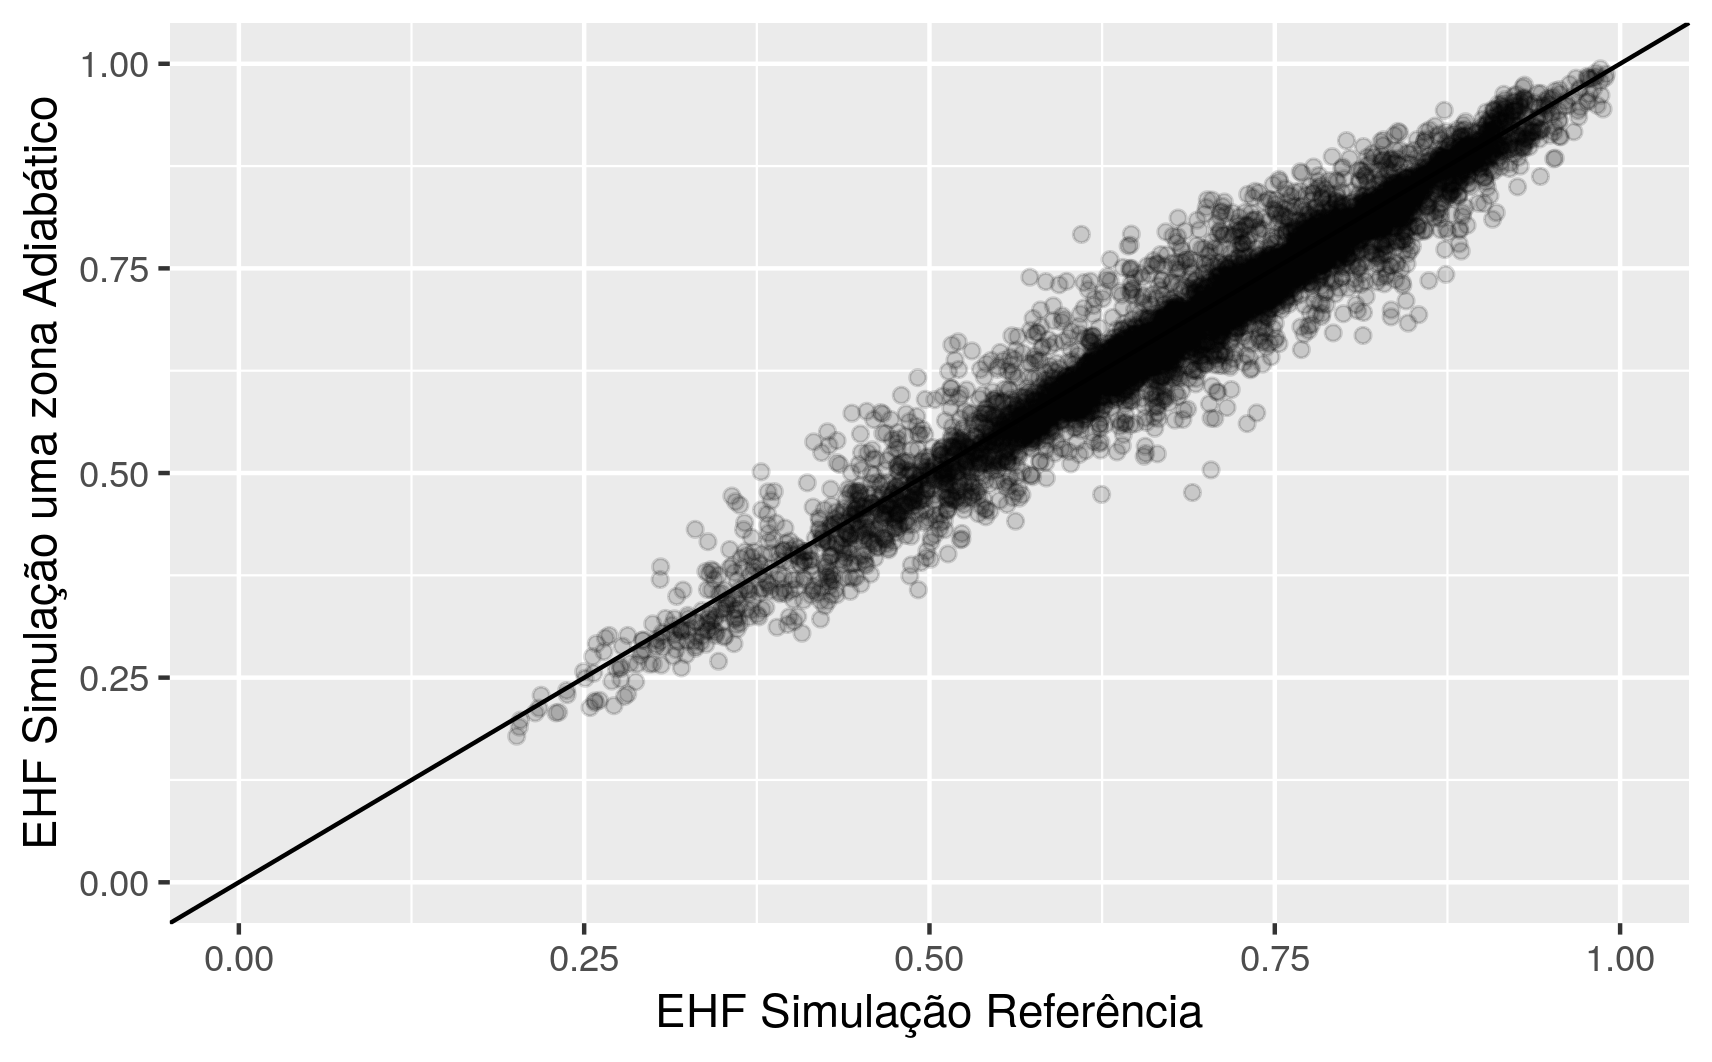
\includegraphics[width=1\linewidth]{img/szadi_EHF_scatter.png}
			\label{fig:szadi_EHF}
			%			\begin{flushleft}
			%				Fonte: o autor.
			%			\end{flushleft}
		\end{figure}
		
		A partir dos resultados obtidos, definiu-se as paredes voltadas para a circulação como adiabáticas, no desenvolvimento das simulações simplificadas.
		
	\subsection{Modelagem da ventilação natural na simulação simplificada}
	
	Nesta etapa do trabalho as simulações foram conduzidas para se obter duas respostas:
	(1) se é adequado o uso do coeficiente de pressão equivalente ($Cp_{eq}$) para ser associado à porta da zona térmica; (2) qual deveria ser o coeficiente de fluxo mássico de ar adotado para o objeto \textit{AirflowNetwork:MultiZone:Surface:Crack}.
	
	Para analisar simultaneamente o desempenho do $Cp_{eq}$ e dos coeficientes de fluxo mássico de ar, o gráfico da Figura \ref{fig:pareto} foi gerado, observando-se as raízes dos erros médios quadráticos (RMSE).
	É possível observar que as simulações desenvolvidas utilizando-se o $Cp_{eq}$ obtiveram resultados com RMSE menores do que as simulações desenvolvidas utilizando-se o Cp obtido diretamente pelo MA.
	Para a definir o coeficiente de fluxo mássico de ar, levou-se em conta inicialmente os erros relacionados às médias dos ACH.
	No entanto, foi identificada uma fronteira de Pareto entre os erros analisados, que mostra como a busca por menores erros de ACH aumento os erros relacionados ao EHF.
	O resultado dessa análise levanta duas hipóteses. A primeira é de que as diferenças maiores nas trocas de ar anulem erros relacionados à definição das paredes adjacentes à edificação como adiabáticas. A segunda hipótese, é de que os maiores erros relacionados ao ACH sejam em casos onde as diferenças nas trocas de ar não sejam relevantes para alterar a temperatura operativa das zonas térmicas e, consequentemente, o EHF.
	
	\begin{figure}[H]
		\centering
		\caption{Eficiência de Pareto entre EHF e ACH}
		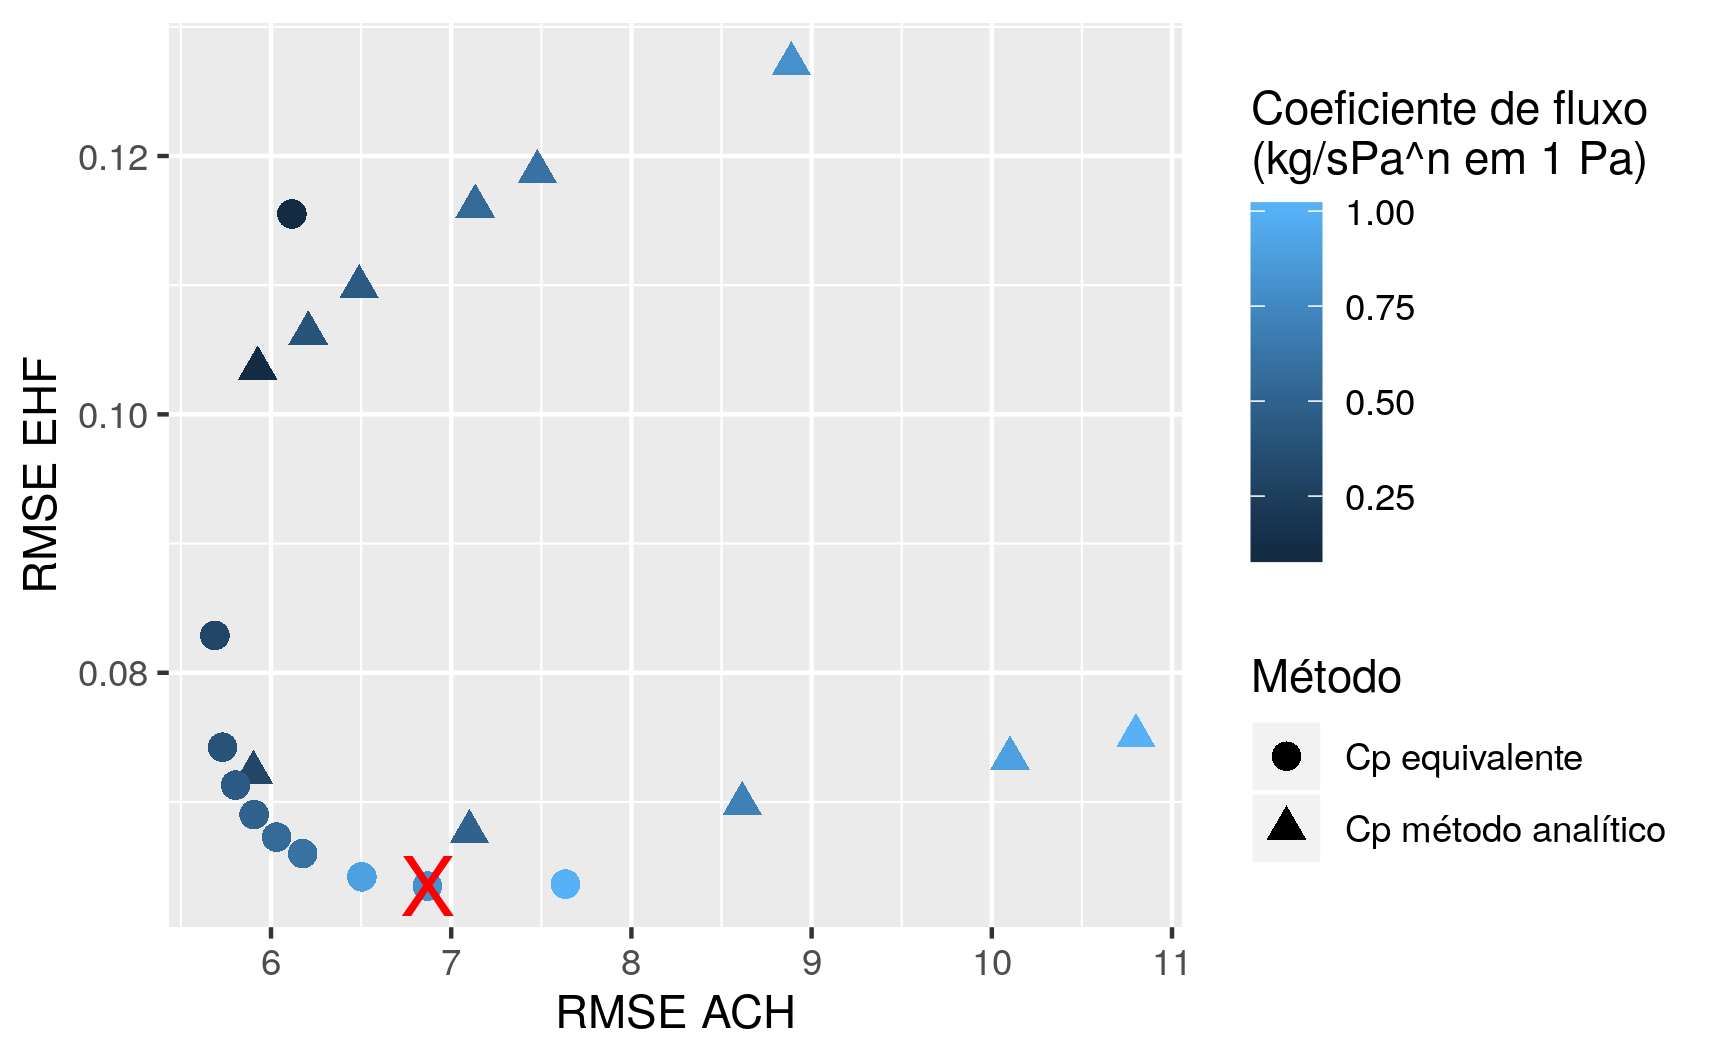
\includegraphics[width=1\linewidth]{img/cpeq_pareto.png}
		\label{fig:pareto}
		%			\begin{flushleft}
		%				Fonte: o autor.
		%			\end{flushleft}
	\end{figure}
	
	Como o desenvolvimento das simulações é voltado para obter a maior precisão possível para os resultados de EHF, optou-se por definir o coeficiente de fluxo mássico de ar com valor igual a 0,8, pois as simulações desenvolvidas utilizando-se este valor estão na fronteira de Pareto, e resultaram nos menores erros de EHF.
	
	\subsection{Análise de sensibilidade}
	
	As Figuras \ref{fig:as_ach}, \ref{fig:as_temp} e \ref{fig:as_ehf} apresentam os resultados das análises de sensibilidade (AS) para efeitos de primeira ordem e efeitos totais, relacionados às médias anuais de ACH, temperaturas operativas das zonas, e EHF. Os índices apresentados são proporcionais às influências entre os dados de entrada e saída.
	
	\begin{figure}[H]
		\centering
		\caption{AS de Sobol dos efeitos de primeira ordem e efeitos totais nas médias anuais de ACH}
		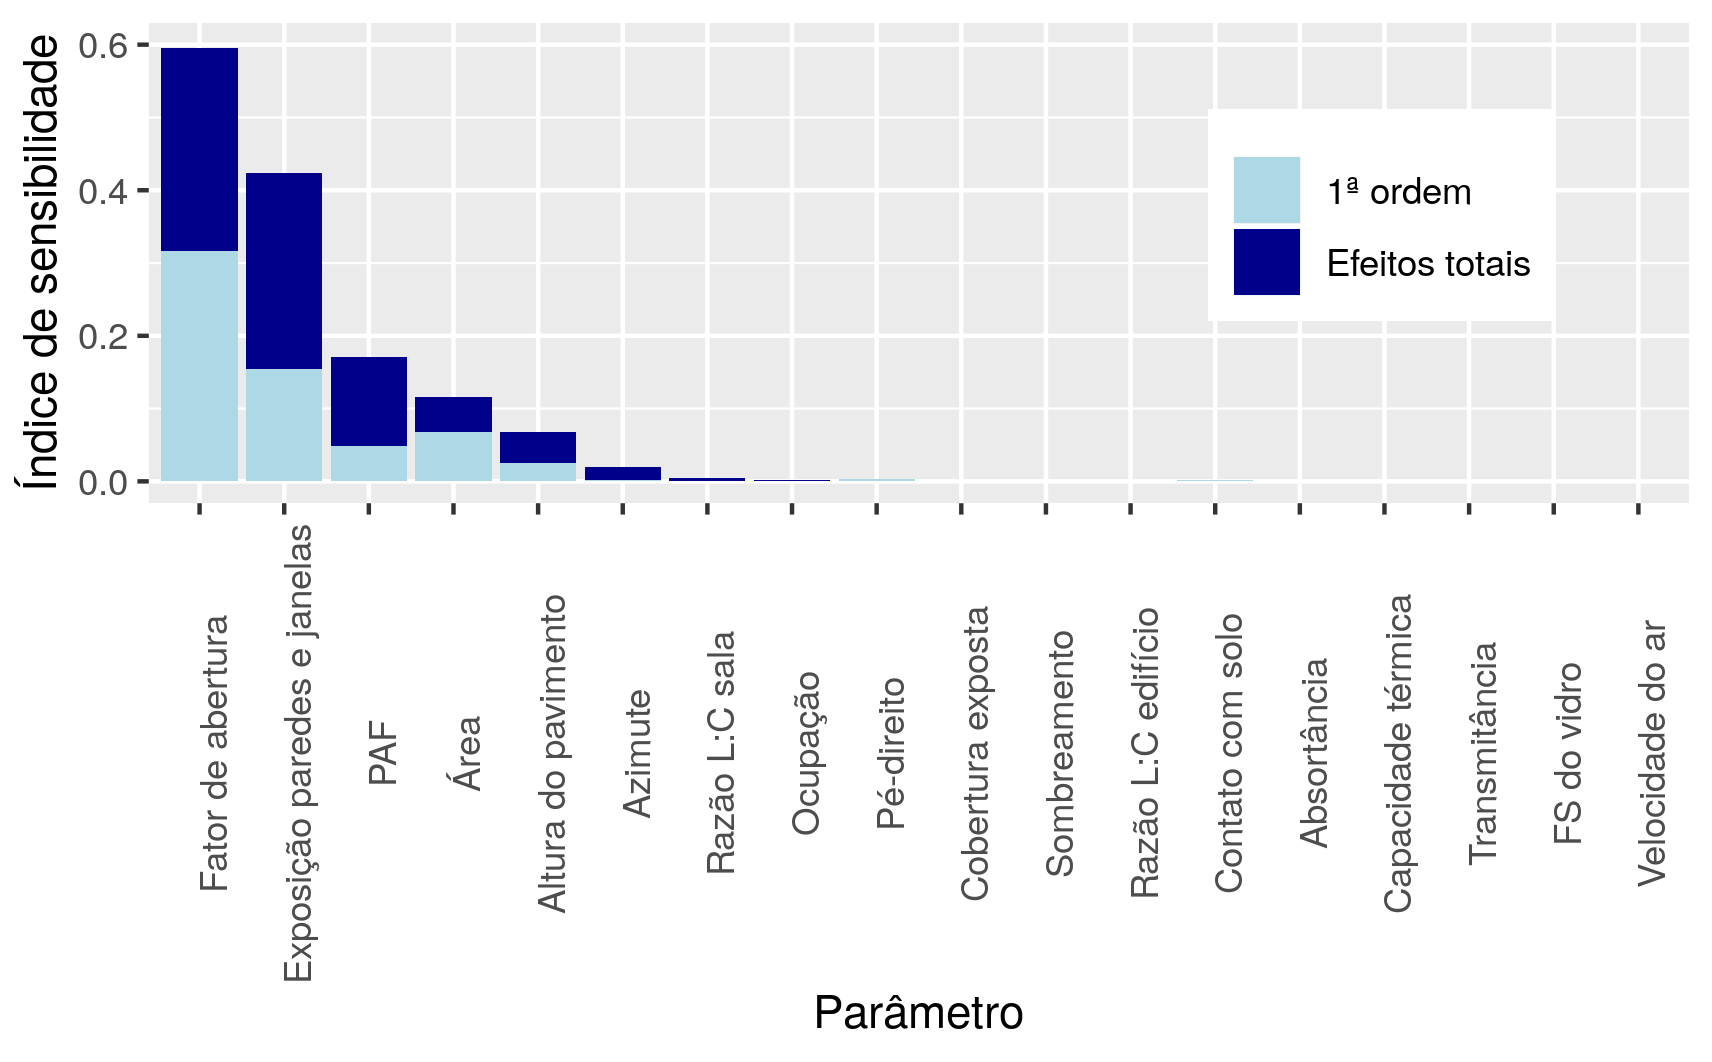
\includegraphics[width=1\linewidth]{img/as_ach.png}
		\label{fig:as_ach}
		%			\begin{flushleft}
		%				Fonte: o autor.
		%			\end{flushleft}
	\end{figure}
	
	\begin{figure}[H]
		\centering
		\caption{AS de Sobol dos efeitos de primeira ordem e efeitos totais nas temperaturas operativas}
		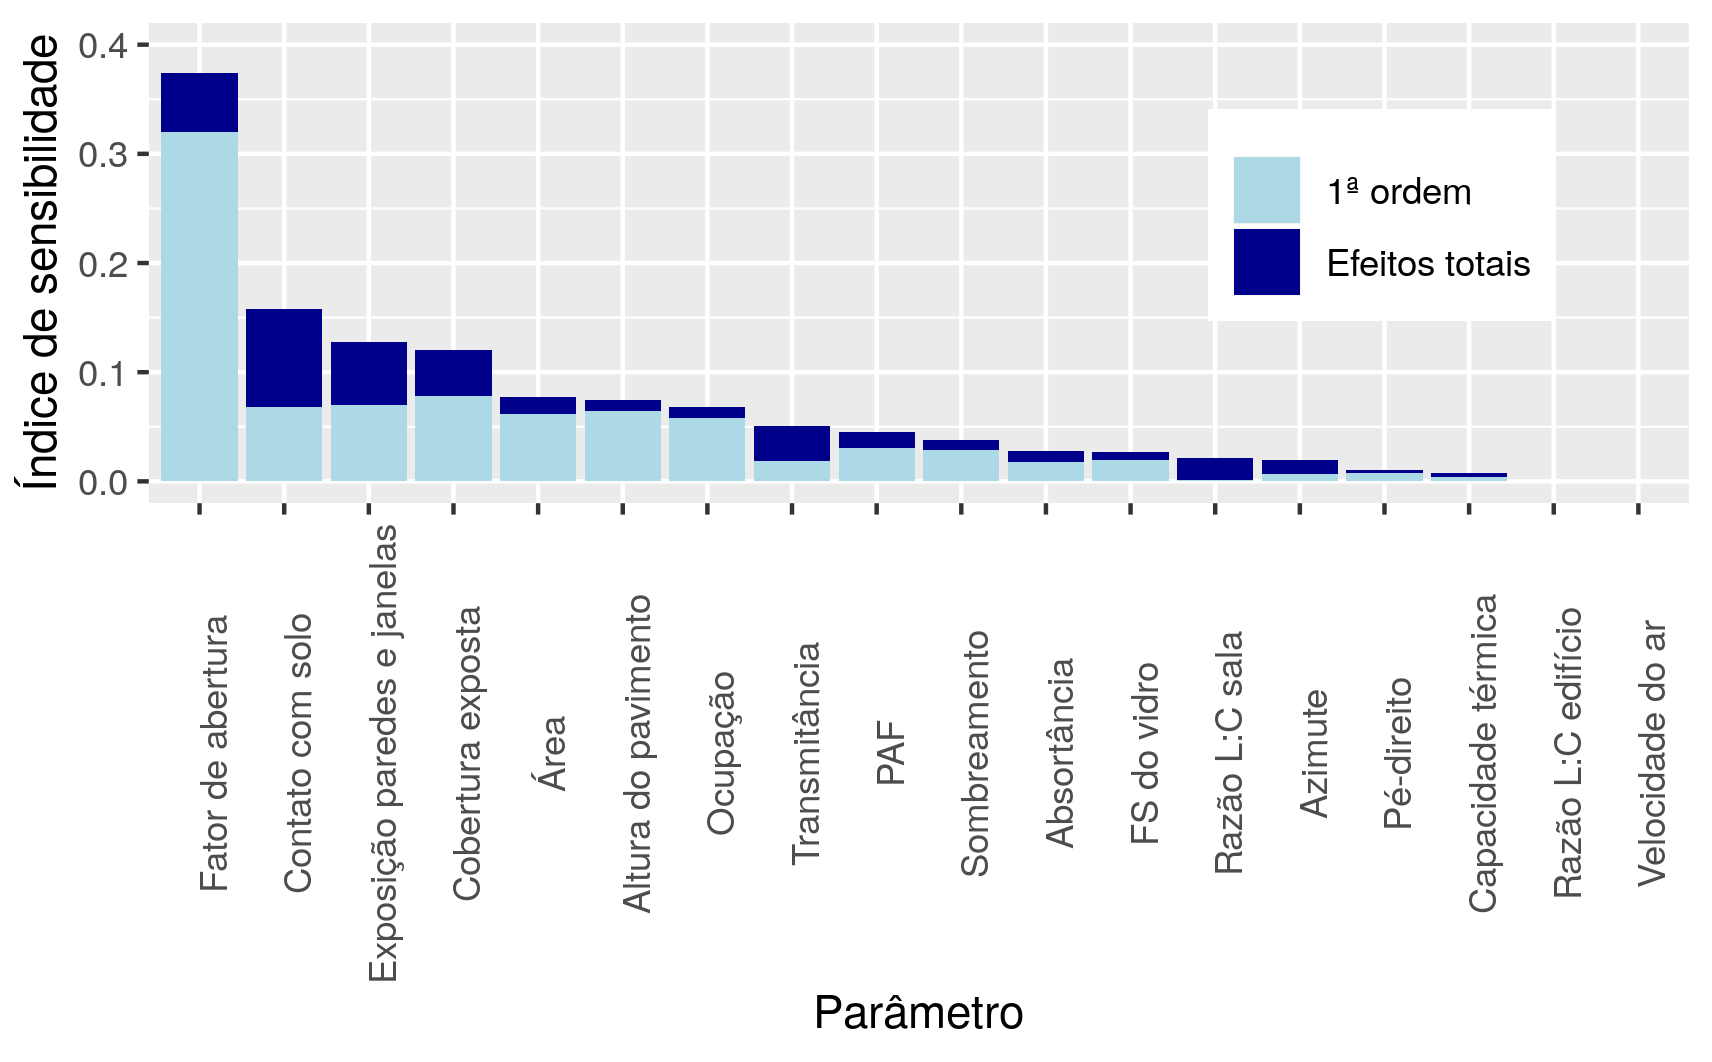
\includegraphics[width=1\linewidth]{img/as_temp.png}
		\label{fig:as_temp}
		%			\begin{flushleft}
		%				Fonte: o autor.
		%			\end{flushleft}
	\end{figure}
	
	\begin{figure}[H]
		\centering
		\caption{AS de Sobol dos efeitos de primeira ordem e efeitos totais no EHF}
		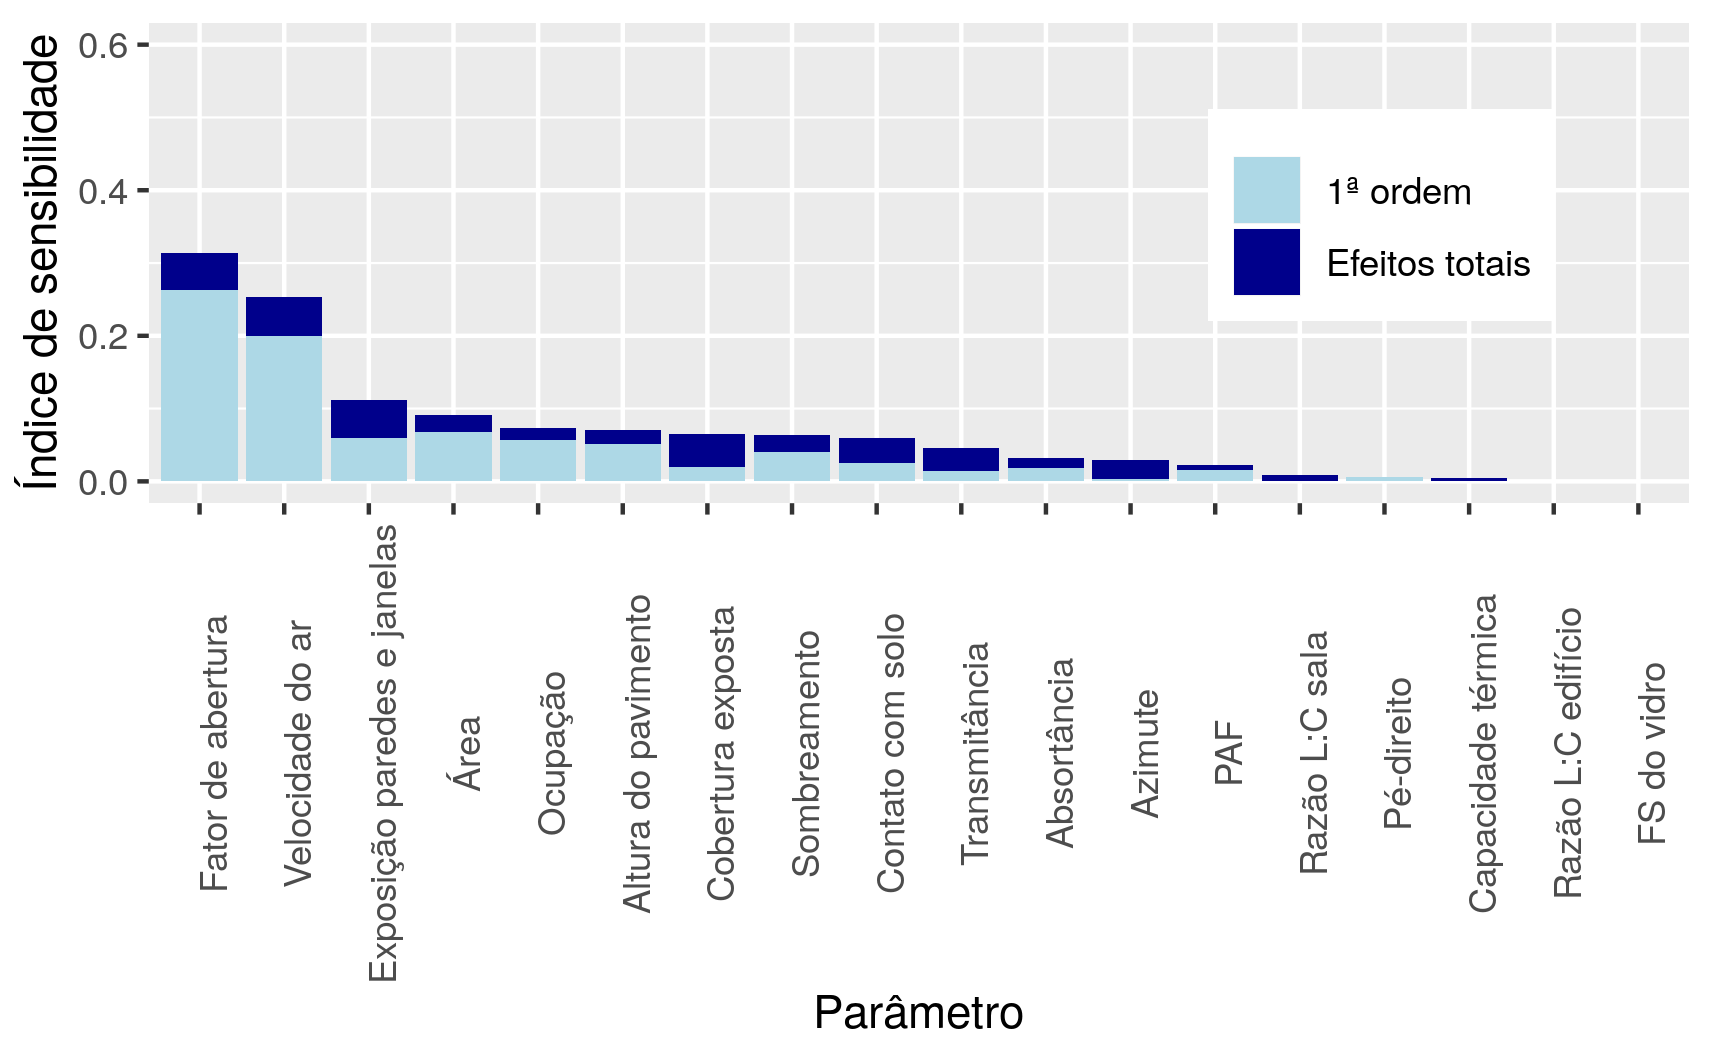
\includegraphics[width=1\linewidth]{img/as_ehf.png}
		\label{fig:as_ehf}
		%			\begin{flushleft}
		%				Fonte: o autor.
		%			\end{flushleft}
	\end{figure}

	Os parâmetros mais influentes nas médias anuais de ACH, como esperado, são aqueles relacionados às aberturas da zona. 
	O primeiro parâmetro de maior influência é o fator de abertura das janelas, seguido do parâmetro relacionado à exposição das paredes e à presença de VN cruzada ou unilateral. A área tem influência significativa, pois o cálculo das trocas de ar leva em conta o volume de ar na zona, que é diretamente relacionado à sua área. 
	A altura do pavimento é determinante nos resultados do ACH, pois a velocidade do vento no EnergyPlus é calculada em função da altura da zona.
	A orientação da zona (azimute) não tem uma influência significativa de primeira ordem. No entanto, percebe-se uma influência mais significativa considerando-se os efeitos totais. O azimute é determinante para determinar os coeficientes de pressão sobre as fachadas da edificação. Por isso, a influência deste parâmetro depende de outros parâmetros, relacionados às áreas e ao posicionamento das aberturas na zona.
	A velocidade do ar não influencia os resultados, pois é considerada apenas após o término das simulações, ao se calcular o EHF.
	
	As análises relacionadas à temperatura operativa e ao EHF indicam a relevância dos parâmetros relacionados à ventilação natural. Para ambas as análises, o parâmetro mais influente foi o fator de abertura da janela, enquanto o parâmetro relacionado à exposição das paredes e à presença de VN cruzada ou unilateral foi o terceiro mais influente. 
	O contato com o solo apresentou-se como o segundo parâmetro mais influente nas médias anuais de temperatura operativa, considerando-se os esfeitos totais. No entanto, a influência deste parâmetro não é tão significativa no EHF. Isso indica que a influência do contato com o solo nas temperaturas operativas das zonas é mais significativa em faixas de temperatura que não interferem no cálculo do EHF, ou seja, consideravelmente a cima ou abaixo dos limites superiores.
	Observa-se que os efeitos totais entre o segundo (contato com o solo) e o quarto (exposição da cobertura) parâmetro definidos como mais influentes na média anual de temperatura operativa são determinantes. Se fossem considerados apenas efeitos de primeira ordem, os índices de sensibilidade seriam muito semelhantes entre o segundo e o nono parâmetro mais influente.
	A transmitância das paredes, o azimute, e a razão entre a largura e o comprimento da sala apresentam baixos índices de sensibilidade para primeira ordem, porém têm efeitos totais relevantes. Isso indica que há colinearidade significativa entre esses parâmetros e os demais.
		
	O movimento do ar apresenta-se como o segundo parâmetro mais influente nos resultados de EHF, o que indica um grande potencial de uso de ventiladores na busca por conforto térmico nos ambientes. 
	A área da zona e a densidade de ocupação apresentaram-se mais influentes nos resultados de EHF, comparando-se aos resultados relacionados às médias anuais de temperatura operativa.
	
	Baseando-se nos resultados das AS, alguns dos parâmetros não foram considerados para o desenvolvimento do metamodelo. A Tabela \ref{table:param_fixed} apresentam os parâmetros que tiveram seus valores fixos. Os valores fixos foram determinados a considerando-se os valores encontrados com mais frequência, com exceção dos parâmetros relacionados às proporções entre largura e profundidade das salas e edifícios, que foram determinados com valor igual a 1. 
	
	\begin{table}[H]		
		\centering
		\caption{Parâmetros com valores constantes.}
		\label{table:param_fixed}
		\begin{tabular}{|l |c |}
			\hline
			\textbf{Parâmetro} & Valor fixo \\
			\hline
			Razão L:C do edifício (-) & 1 \\
			\hline
			Razão L:C da sala (-) & 1 \\
			\hline
			Pé-direito (m) & 2,5 \\
			\hline
			Capacidade térmica (kJ/m$^2$K) & 161 \\
			\hline
			Fator solar do vidro (-) & 0,87 \\
			\hline
		\end{tabular}
	\end{table}
	
%	Occupant density is the most influential parameter
%	on EHF, since it obtained the highest index value for
%	first order, second order and total effects. From the
%	first order effects indices, it was observed that, after
%	occupant density, the contact with the ground and
%	the window opening factor are the most influential
%	parameters on both EHF and average Operative Tem-
%	perature. The index values for these two outputs are
%	similar overall, since EHF is calculated from the Op-
%	erative Temperature. Therefore, the annual average
%	Operative Temperature results were not plotted. The
%	most influential parameters on the ACH are, as ex-
%	pected, the ones related to the zone’s openings. They
%	are: opening factor of the window; exposure condition
%	of walls and windows; and WWR.
%	Significant colinearities are identified among the pa-
%	rameters. Even though the zone area has a higher
%	first order index, the exposure of the walls and the
%	roof could be more influential on the EHF, when com-
%	bined with certain parameters. Second order effects
%	analysis shows high interaction between the exterior
%	walls exposure and the opening factor of the win-
%	dow. The interaction could be explained due to the
%	the higher influence of either one or two windows on
%	the facade when the window opening factor is higher.
%	The highest second order effect index for EHF was
%	the one relating occupant density and ground expo-
%	sure. These two parameters were also the two most
%	influential for first order and total effects analyses.
%	
%	Thus, this strong relation points out how contact with
%	the ground can help to dissipate internal heat gains
%	at the climate of Sao Paulo.
%	Based on the SA results, some the least influential
%	parameters were not considered as input features for
%	the final model. They are: height of the zone’s floor;
%	SHGC; wall thermal capacity; shading device; build-
%	ing ratio.

	\subsection{Desenvolvimento do metamodelo}
	
	A partir das 100.000 simulações geradas para o treinamento da rede neural artificial (RNA), obteve-se resultados de EHF variando entre 0,00 e 1,00.
	
	O metamodelo final foi definido com 13 parâmetros:
	\begin{itemize}
		\item Fator de abertura das janelas;
		\item Velocidade do ar;
		\item Condição de exposição das paredes e janelas;
		\item Área da sala;
		\item Densidade de ocupação;
		\item Altura do pavimento;
		\item Exposição da cobertura;
		\item Sombreamento horizontal;
		\item Contato com o solo;
		\item Transmitância das paredes;
		\item Absortância das paredes;
		\item Azimute da sala;
		\item PAF.
	\end{itemize}
	
	Os parâmetros variaram na mesma faixa de valores estabelecida na primeira etapa deste estudo. O ângulo do azimute da sala é determinado considerando-se o eixo entre a porta e a janela em frente à porta.
	
	O contato com o solo e a exposição da cobertura foram definidas como variáveis binárias, com o valor zero correspondendo à superfície adiabática, e 1 correspondendo à exposição.
	O parâmetro que representa a condição de exposição das paredes e janelas não foi representado com valores numéricos, e sim como uma variável de fatores, com cinco opções de exposição. Além das três opções apresentadas na Figura \ref{fig:exp_sz}, considerou-se as exposições espelhadas. 	
	Os demais parâmetros foram normalizados com valores entre -1 e 1.
	
	\begin{figure}[H]
		\centering
		\caption{Condição de exposição das paredes e janelas.}
		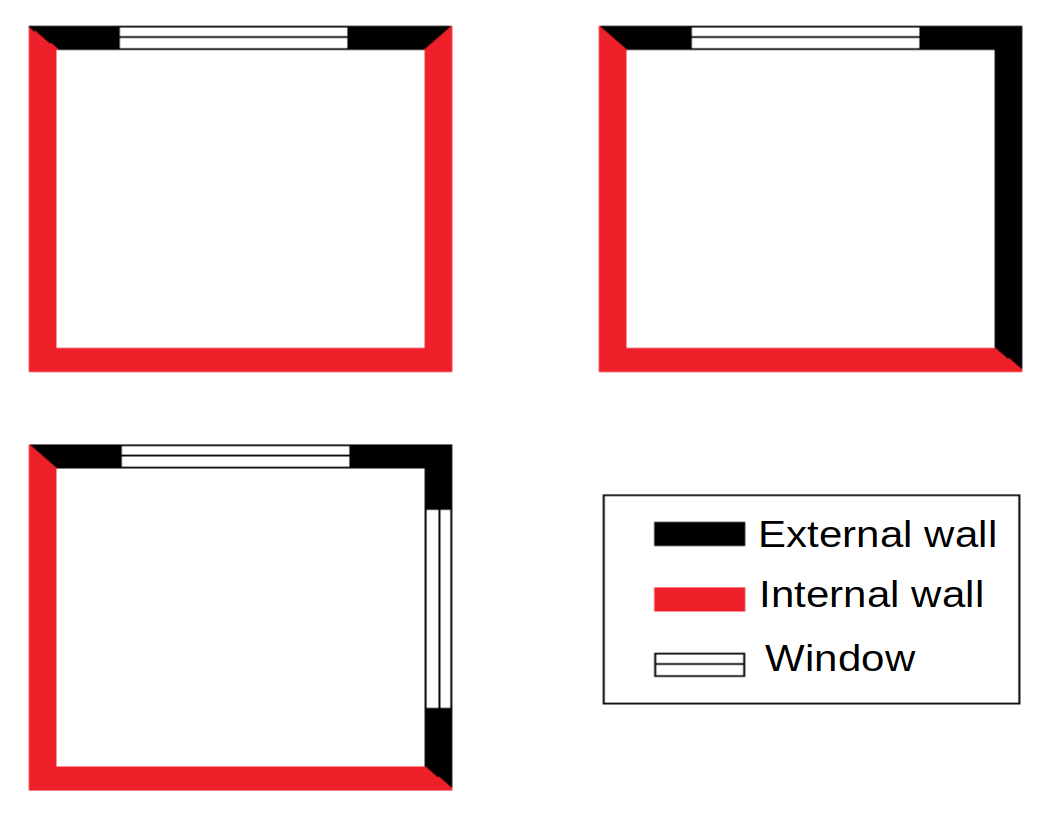
\includegraphics[width=1\linewidth]{img/wallexposition.png}
		\label{fig:exp_sz}
		%			\begin{flushleft}
		%				Fonte: o autor.
		%			\end{flushleft}
	\end{figure}
	
	O modelo de RNA final foi definido com duas camadas, umas de 50 nós, e a outra com 20. 
	O algorítimo de otimização que obteve o melhor desempenho foi o \textit{Adagrad's Optimizer}, disponibilizado pela biblioteca \textit{TensorFlow}, com uma taxa de aprendizagem igual a 0,05.
	
	A Figura \ref{fig:ann_validation} apresenta um gráfico de pontos comparando os resultados de EHF obtidos para as simulações e para as estimativas da RNA, a partir da base de dados desenvolvida para a validação do metamodelo. A base de dados para a validação teve apenas os parâmetros incluídos no treinamento da RNA variados. 
	O erro absoluto médio do EHF para os casos de validação foi 0,0104, com o AE95 igual a 0,0226.
	
	\begin{figure}[H]
		\centering
		\caption{Condição de exposição das paredes e janelas.}
		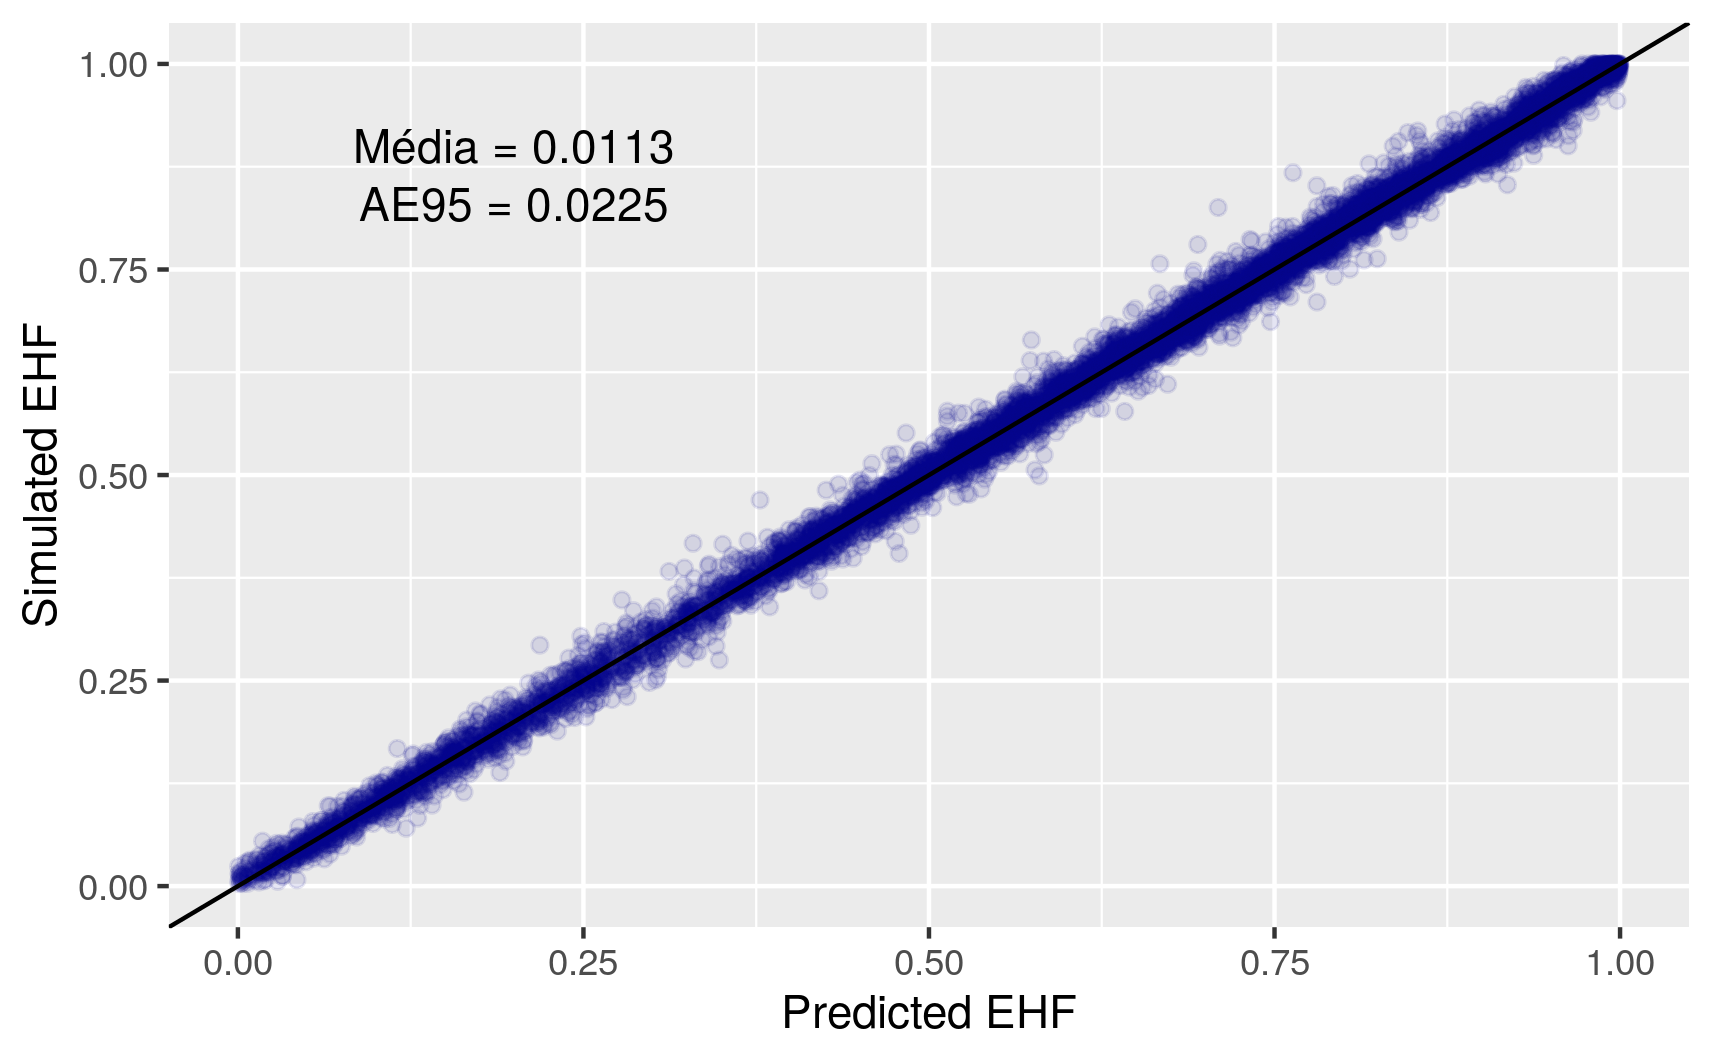
\includegraphics[width=1\linewidth]{img/ann_validation.png}
		\label{fig:ann_validation}
	\end{figure}
	
	Outra comparação foi conduzida com a amostragem utilizada para a AS. Essa base de dados estava disponível, e não foi utilizada pra o desenvolvimento da RNA, então ela foi escolhida para testar o desempenho da RNA quando todos os parâmetros avaliados neste estudo variam. A Figura \ref{fig:ann_sobol} apresenta o gráfico de pontos comparando os resultados de EHF obtidos para as simulações e para as estimativas da RNA, a partir da base de dados da AS de sobol. O erro absoluto médio do EHF para os casos de validação foi 0,0104, com o AE95 igual a 0,0226.
	
	\begin{figure}[H]
		\centering
		\caption{Condição de exposição das paredes e janelas.}
		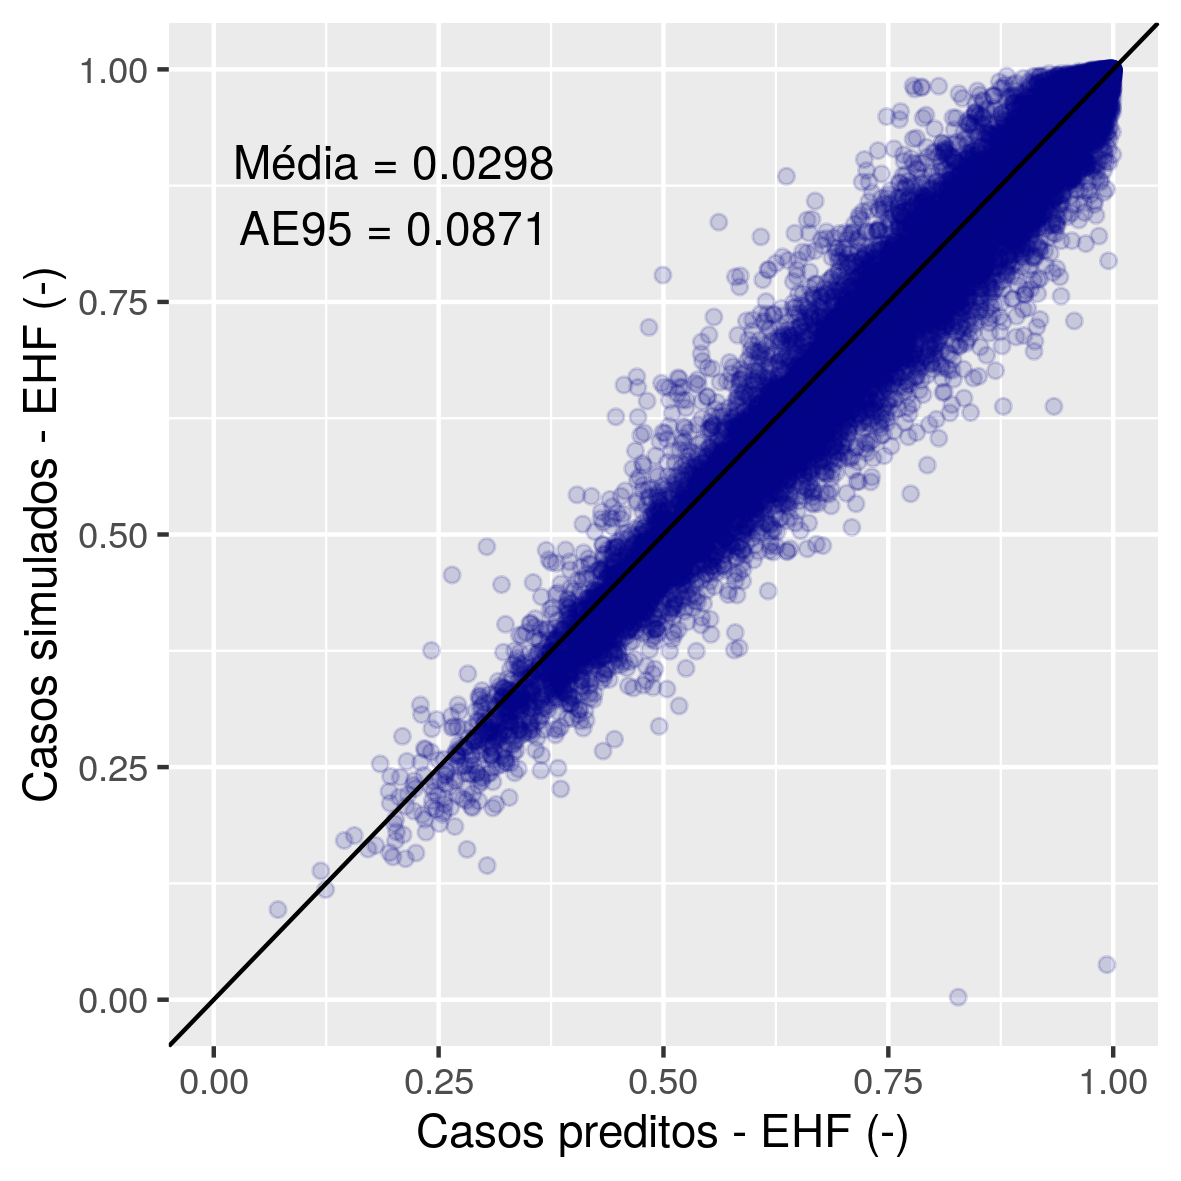
\includegraphics[width=1\linewidth]{img/ann_test.png}
		\label{fig:ann_sobol}
	\end{figure}
	
	

\bibliography{citacoes}
	
\end{document}